\chapter{Resultados y discusi\'on}
\label{ch:resAuger}

Una vez definidos los criterios de selección es posible calcular la exposición del detector y llevar a cabo la búsqueda de candidatos.



\section{C\'alculo de la exposici\'on}
\label{sc:expoNu}
	
	La exposición es una cantidad comunmente utilizada en física de astropartículas para caracterizar una medición.
	Se la define como la magnitud que, convolucionada con un flujo de partículas $\frac{dN_{\nu}}{d\Gamma}$, resulta en la cantidad de eventos que se espera haber detectado durante la misma, como se muestra en la ecuación \ref{eq:exp0}.
	%
	\begin{equation}
	 N_{esp}=\int\limits_{\Gamma}~\frac{dN_{\nu}}{d\Gamma}~\mathscr{E}(\Gamma) ~d\Gamma
	 \label{eq:exp0}
	\end{equation}
	%
	En esta, $\Gamma$ simboliza el conjunto de variables del que dependa la detección, que en este trabajo corresponde a $(E_{\nu},A,\Omega,T)$\footnote{Se desprecia cualquier tipo de inhomogeneidad en el flujo.}, es decir, la energía de los neutrinos incidentes, el área del detector, el ángulo sólido que se observa y el tiempo durante el que se mide, respectivamente.
	
	De la ecuación \ref{eq:exp0} se desprende entonces que, como $\frac{dN_{\nu}}{d\Gamma}$ es la cantidad de neutrinos de energía $E_{\nu}$ que alcanzan el detector por unidad de área, ángulo sólido y tiempo, la exposición debe representar qué cantidad de cada energía se espera haber detectado en promedio en cada unidad de área del detector y en cada instante de tiempo.
	Es decir, la exposición contiene toda la información correspondiente a la medición y al detector, mientras que el flujo incluye la física de la fuente de lo que se espera detectar.
	
	Si se considera a $\frac{dN_{\nu}}{d\Gamma}$ como un flujo difuso $\Phi(E_{\nu})$, es decir isótropo, homogeneo y constante en el tiempo, la ecuación \ref{eq:exp0} puede escribirse como \ref{eq:exp1}.
	%
	\begin{equation}
	 N_{esp}=\int\limits_{E_{\nu}}~\Phi(E_{\nu})\left[~\iiint\limits_{T~\Omega~A}\mathscr{E}(E_{\nu},A,\Omega,T) ~dA~d\Omega~dT~\right]~dE_\nu
	 \label{eq:exp1}
	\end{equation}
	%
	La función de $E_\nu$ entre corchetes, que corresponde a la exposición integrada en el caso de un flujo difuso, será llamada de aquí en más \emph{exposición del detector} y será simbolizada por la letra $\cal E$, como se muestra en la ecuación \ref{eq:exp2}.
	%
	\begin{equation}
	 {\cal E}(E_\nu)\equiv\iiint\limits_{T~\Omega~A}\mathscr{E}(E_{\nu},A,\Omega,T) ~dA~d\Omega~dT
	 \label{eq:exp2}
	\end{equation}
	%
	El objetivo a partir de aquí es la construcción de esta cantidad que requiere de los siguientes ingredientes:
	\begin{enumerate}
	 \item La probabilidad de que un neutrino de energía $E_\nu$ proveniente del sector $\Omega$~\footnote{Es decir, cuya dirección se caracteriza por los ángulos $(\theta,\phi)$.} de inicio a una lluvia atmosférica extendida de parámetros $X$.
	 \item La probabilidad de que una lluvia de parámetros $X$ dispare el detector y que el evento registrado sea identificado como un neutrino, es decir, las eficiencias de identificación.
	 \item La integración de estas probabilidades sobre el área del detector, el tiempo de medición, las diferentes direcciones de arrivo y las distintas lluvias atmosféricas que se puedan generar.
	\end{enumerate}
	
	Teniendo esto en cuenta, la ecuación \ref{eq:exp2} puede escribirse como en la ecuación \ref{eq:exp3}.
	%
	\begin{equation}
	 {\cal E}(E_\nu)\equiv\iiiint\limits_{T~\Omega~A~X}P(X|E_{\nu},A,\Omega,T)~\epsilon(X,E_{\nu},A,\Omega,T) ~dX~dA~d\Omega~dT
	 \label{eq:exp3}
	\end{equation}
	% 
	Según lo que se expuso en la sección \ref{sc:libGen} para eventos ES el parámetro $X$ debe corresponder al conjunto $(E_\tau,{\rm x_d})$, mientras que en el caso de DG corresponde a la profundidad inclinada de interacción $D$.
	Por otro lado, la probabilidad de ocurrencia de un evento de parámetros $X$ simplemente incluye la información del blanco con el que los neutrinos interactúan: la tierra en ES y la atmósfera en DG. 
	En ambos casos en este trabajo se desprecian las fluctuaciones que estos puedan tener durante el tiempo que dura la medición o al variar la fracción del detector que se esté estudiando, por lo que $P(X|E_{\nu},A,\Omega,T)~\rightarrow~P(X|E_{\nu},\Omega)$.
	Incuyendo toda esta información, para calcular la exposición del detector habrá que realizar las integrales de las ecuaciones \ref{eq:exp4DG} y \ref{eq:exp4ES}.
	%
	\begin{equation}
	 {\cal E}_{DG}(E_\nu)\equiv\iint\limits_{D~\Omega}P(D|E_{\nu},\Omega)~
	 \left[~
	 \iint\limits_{T~A}\epsilon(D,E_{\nu},A,\Omega,T)~dA~dT
	 \right]
	 ~d\Omega~dD
	 \label{eq:exp4DG}
	\end{equation}
	%
	\begin{equation}
	 {\cal E}_{ES}(E_\nu)\equiv\iiint\limits_{E_\tau~{\rm x_d}~\Omega}P({\rm x_d},E_\tau|E_{\nu},\Omega)~
	 \left[~
	 \iint\limits_{T~A}\epsilon({\rm x_d},E_\tau,A,\Omega,T)~dA~dT
	 \right]
	 ~d\Omega~d{\rm x_d}~dE_\tau
	 \label{eq:exp4ES}
	\end{equation}
	%
	
	En las siguientes secciones se abordará la obtención de cada uno de los términos.
	
	\subsection{Término de probabilidad}
	
	El término de probabilidad conecta el flujo con las eficiencias en el cálculo de la exposición.
	En este caso, el flujo representa la cantidad de eventos que se esperan por unidad de área, tiempo y ángulo sólido, mientras que por construcción las eficiencias corresponden a la cantidad de eventos detectados segun variables relacionadas con el proceso de medición\footnote{$(E_\tau,\Omega,{\rm x_d})$ en ES y $(E_\nu,\Omega,D)$ en DG.}.
	Entonces, coloquialmente este término responde a la prgunta: ¿cuántos de los eventos que predice el flujo espero en cada bin en que conozco la eficiencia?
	
	\subsubsection{Eventos DG}
	
	Como se expuso en la sección \ref{sbsc:easDG}, el camino libre medio de los neutrinos es varios órdenes de magnitud mayor que el espesor de la atmósfera, por lo que es una muy buena aproximacion considerar la probabilidad de interacción una constante para cualquier profundidad de interacción, o lo que es lo mismo, que la magnitud del flujo no depende de la misma.
	Con esto en mente, para obtener la expresión de $P(D|E_{\nu},\Omega)$ es útil primero considerar un caso simplificado: un haz de partículas, con flujo lineal~$F$ (medido en partículas por unidad de área por unidad de tiempo), que incide sobre un blanco con~$N$ elementos dispersores. En esta situación la cantidad de colisiones~$n$ por unidad de tiempo está dada por:
	%
	\begin{equation}
	% \frac{\Delta n}{\Delta t} 
	n = F\,\sigma\,N
	\end{equation}
	% 
	en donde $\sigma$ es la sección eficaz de interacción entre las partículas del haz y las del blanco.
	Si se considera un blanco de masa~$M$ formado por elementos dispersores de masa~$m$ el número de colisiones por unidad de tiempo es simplemente:
	%
	\begin{equation}
	% \frac{\Delta n}{\Delta t} 
	n = F\,\sigma\,\frac{M}{m}
	\end{equation}
	% 

	El resultado anterior se puede extender para analizar el caso de un flujo diferencial difuso~$\Phi(E_{\nu})$ y un detector plano que registra todas las lluvias producidas por neutrinos que satisfacen las siguientes condiciones  (ver figura \ref{fig:diferencialMasa}):
	%
	\begin{itemize}
	\item su dirección de arrivo apunta a una región $\Delta A$ del detector ubicada en $\vec{r}$
	\item su dirección de arrivo $(\theta,\phi)$ está en un rango 
	$\Delta \Omega=\sen\theta\,\Delta\theta\,\Delta\phi$
	\item su energía~$E_{\nu}$ está en un rango $\Delta E_{\nu}$
	\item interactúa a una profundidad másica~$D$ en el rango $[D, D+\Delta D]$. 
	\end{itemize}
	%
	En este caso el número de lluvias observadas por unidad de tiempo está dado por
	%
	\begin{equation}
	% \frac{\Delta \mathfrak{N}}{\Delta t}
	n = \Phi(E_{\nu})\, \Delta E_{\nu}\,\Delta\Omega\;\sigma(E_{\nu})\;\frac{\Delta M}{m}
	\label{eq:dn_domega}
	\end{equation}
	%
	donde la cantidad de masa $\Delta M$ contenida en un espesor $\Delta D $ depende del ángulo cenital, $\Delta M= \Delta D \, \Delta A \, \cos\theta$ (ver figura \ref{fig:diferencialMasa}). La profundidad másica $D$ tiene unidades de masa sobre área. Para el caso del Observatorio Auger, en Malarg\"ue, el espesor másico de la atmósfera vertical es de 860 g/cm$^2$.
	%  
	\begin{figure}[ht]
	\begin{center}$
	\begin{array}{cc}
	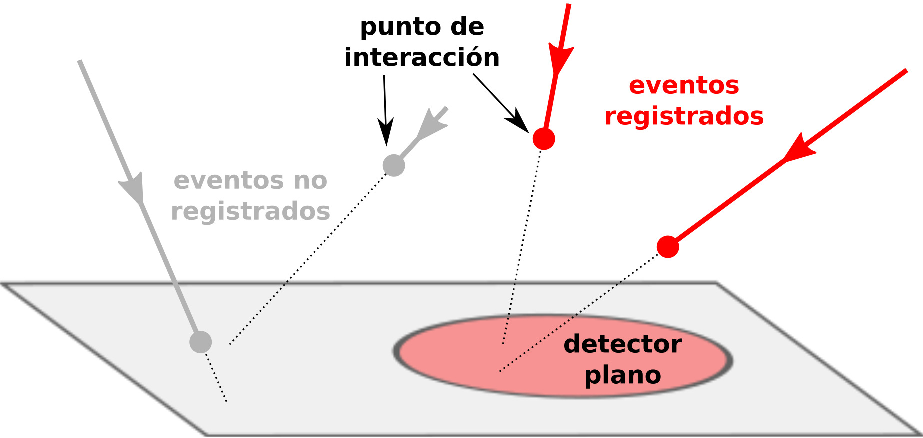
\includegraphics [width=0.52\textwidth]{fig/resultadosAuger/detectorPlano.pdf} & 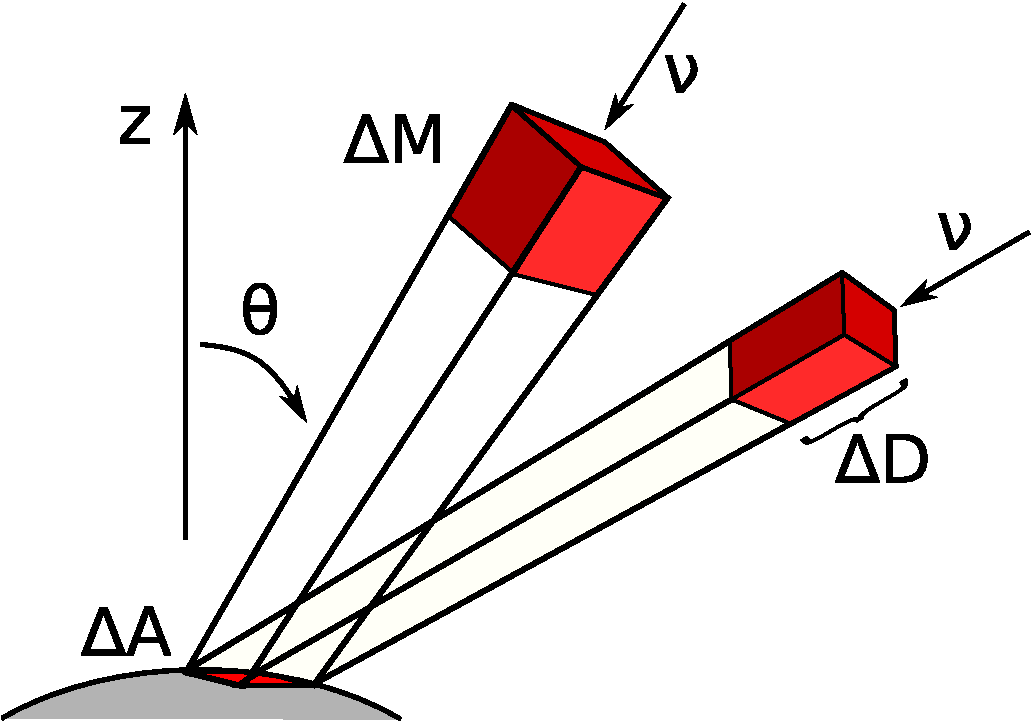
\includegraphics [width=0.42\textwidth]{fig/resultadosAuger/diferencialMasa.pdf}
	\end{array}$
	\end{center}
	\caption{
	\textit{Panel izquierdo}: vista esquemática de un detector plano imaginario que registra todos los eventos producidos por partículas cuya dirección de arrivo cruza su superficie. \textit{Panel derecho}: diagrama de diferencial de masa $\Delta M$ según se define en el texto. Puede observarse que $\Delta M$ crece al disminuir el ángulo cenital $\theta$.
	}
	\label{fig:diferencialMasa}
	\end{figure}
	%
	
	Si el detector tiene una eficiencia~$\epsilon$ menor que uno, sólo una fracción de las lluvias serán detectadas. En el caso más general~$\epsilon$ es función de $E_{\nu}$, $\theta$, $D$, $\vec{r}$ y $\phi$:
	%
	\begin{equation}
	n = \frac{1}{m}\,\Phi(E_{\nu})\,\sigma(E_{\nu})\,\Delta E_{\nu}\,\Delta D\,\Delta A\,\cos\theta\sen\theta\,\Delta\theta\,\Delta\phi\;\epsilon(E_{\nu},\theta,D,\vec{r},\phi)
	\label{eq:dN_domega}
	\end{equation}
	%
	Integrando en $\phi$ tenemos:
	%
	\begin{equation}
	n = \frac{1}{m}\,\Phi(E_{\nu})\,\sigma(E_{\nu})\,\Delta E_{\nu}\,\Delta D\,\Delta A\,\cos\theta\sen\theta\,\Delta\theta\,2\pi\;\epsilon(E_{\nu},\theta,D,\vec{r})
	\label{eq:dN_domega2}
	\end{equation}
	%
	donde $\epsilon(E_{\nu},\theta,D,\vec{r}) = \frac{1}{2\pi}\int \epsilon(E_{\nu},\theta,D,\vec{r},\phi)\,\d\phi$ es el promedio de la eficiencia respecto del ángulo azimutal. 

	Si se mide durante un tiempo $T$, sumando las contribuciones de todos los bines, pasando a forma integral y reacomodando la ecuación \ref{eq:dN_domega2} se obtiene:
	%
	\begin{equation}
	N = \int\limits_{E_\nu}\Phi(E_{\nu})~
	\tilde{\cal E}_{DG}(E_{\nu})
	~dE_\nu
	\label{eq:dN_domega3}
	\end{equation}
	%
	donde:
	%
	\begin{equation}
	\tilde{\cal E}_{DG}(E_{\nu})
	\equiv 2\pi\iint\limits_{D~\theta}\frac{1}{m}~\sigma(E_{\nu})\cos\theta
		\left[
			~\iint\limits_{T~A} \epsilon(E_{\nu},\theta,D,A)~dA~dT
		\right]
		\sen\theta~d\theta~dD
	\label{eq:dN_domega4}
	\end{equation}
	
	Por otro lado, si se desarrolla el término $d\Omega$ y se integra en $\phi$ en la ecuación \ref{eq:exp4DG} se obtiene:
	\begin{equation}
	{\cal E}_{DG}(E_\nu)\equiv2\pi\iint\limits_{D~\theta}P(D|E_{\nu},\theta)~
	 \left[~
	 \iint\limits_{T~A}\epsilon(D,E_{\nu},A,\theta,T)~dA~dT
	 \right]
	 \sen\theta~d\theta~dD
	\label{eq:exp5DG}
	\end{equation}
	
	Entonces, por comparación entre \ref{eq:dN_domega4} y \ref{eq:exp5DG} se tiene como se esperaba, que $P(D|E_{\nu},\theta)$ es una constante y vale:
	\begin{equation}
	 P(D|E_{\nu},\theta) = \frac{1}{m}~\sigma(E_{\nu})\cos\theta
	\end{equation}
	
	En este trabajo se utilizó la sección eficaz neutrino nucleón dada en \cite{cite:cooper_sarkar}.
	
	\subsubsection{Eventos ES}
	
	La expresión de este término en el caso de los eventos ES es algo mas complicada debido a que el proceso de detección consta de dos pasos:
	\begin{enumerate}
	 \item La primer interacción dentro de la tierra y la propagación hasta el escape.
	 \item La propagación en la atmósfera hasta su decaimiento.
	\end{enumerate}
	
	En la sección \ref{sc:pesos} se analizó cada uno de estos pasos para corregir los pesos de las simulaciones de neutrinos ES.
	La inclusión de la propagación dentro de la tierra se realizó mediante simulaciones de montecarlo, como se detalló en la sección \ref{sbsbsc:sim_prop_tierra}.
	A partir de estas se obtuvo el término $f(E_\tau|E_\nu,\theta)$, que representa la densidad de probabilidad de la energía de los \tauon{}'s que escapande la tierra si los neutrinos incidentes tienen energía \enu{} y ángulo cenital $\theta$.
	Por otro lado, la incorporación de la probabilidad de decaimiento del \tauon{} en la atmósfera también se analizó en la sección \ref{sc:pesos} y esta dada por la ecuación:
	%
	\begin{equation}
		h(x_d,(E_\tau,\theta))=
		\exp{\left(
		-\frac{x_d}{|\cos\theta|\lambda(E_\tau)}
		\right)}
		\frac{1}{|\cos\theta|\lambda(E_\tau)}
	\end{equation}
	%
	Finalmente, es necesario incluir el término que tiene en cuenta la variación del diferencial de volumen en el que se produce la interacción con el ángulo cenital, $|\cos\theta|$.
	
	Con todo esto, desarrollando la integral en $\Omega$ e integrando en $\phi$ la ecuación \ref{eq:exp4ES} queda:
	%
	\begin{equation}
	\begin{aligned}
	 {\cal E}_{ES}(E_\nu)\equiv2\pi\iiint\limits_{E_\tau~{\rm x_d}~\theta}P({\rm x_d},E_\tau|E_{\nu},\theta)~
	 \left[~
	 \iint\limits_{T~A}\epsilon({\rm x_d},E_\tau,A,\theta,T)~dA~dT
	 \right]\\
	 ~\sen\theta d\theta~d{\rm x_d}~dE_\tau
	 \end{aligned}
	 \label{eq:exp5ES}
	\end{equation}
	%
	donde:
	\begin{equation}
	 P({\rm x_d},E_\tau|E_{\nu},\theta)=
	 f(E_\tau|E_\nu,\theta)
	 h(x_d,(E_\tau,\theta))
	 |\cos\theta|
	\end{equation}
	
	\subsection{Eficiencias de identificación en un detector infinito}
	\label{sbsc:idealEff}
	
	Para construir las eficiencias en un detector real es útil estidiarlas antes sobre un detector ideal.
	Mientras que el detector real no solo es finito sino que su forma puede variar en el tiempo, por ejemplo debido a que es común que las estaciones entren y salgan de servicio, un detector ideal consiste en una representación infinita y regular del verdadero.
	Entonces, para obtener las eficiencias de identificación de cada uno de los análisis se simuló una copia del SD de Auger de \cant{50\times50}{km}, infinita a los fines prácticos\footnote{Ningún eventos simulado supera los \cant{25}{km} de extensión.}, se lanzó sobre su centro lluvias simuladas y se obtuvo la señal en el detector tal como se explicó en la sección \ref{sc:offline}.
	Luego, se aplicaron los criterios de identificación de neutrinos desarrollados en el capítulo \ref{ch:selAuger} y se calculó la eficiencia en cada bin con la siguiente ecuación:
	%
	\begin{equation}
	 \epsilon_\chi(X)=\frac{N_{\chi}(X)}{N_{sim}(X)}
	 \label{eq:effDef}
	\end{equation}
	%
	donde $X$ es la etiqueta del bin, mientras que $N_{\chi}$ y $N_{sim}$ son la cantidad de lluvias que se identificaron con el criterio $\chi$ y simularon en el mismo. En nuestro análisis $\chi$ puede representar el nivel de disparo T3 del detector, la clasificación de  evento inclinado y la identificación como neutrino.
	
	\subsubsection{Eficiencias a neutrinos DG}
	
	La eficiencia a neutrinos DG depende de los siguientes parámetros:
	%
	\begin{itemize}
	 \item la profundidad de interacción $D$
	 \item el ángulo cenital $\theta$
	 \item la energía del neutrino $E_\nu$
	 \item sabor del neutrino $(e,\mu,\tau)$
	 \item tipo de interacción (CC o CN)
	\end{itemize}
	%
	Por otro lado, si bien esta también podría depender del ángulo azimutal $\phi$, al haberse simulado de manera aleatoria, la eficiencia obtenida en cada bin de $(E_\nu,\theta,D)$ y para cada sabor y canal, será un promedio en el ángulo azimutal.
	
	La figura \ref{fig:effDG_tr_id} muestra la eficiencia de disparo T3 e identificación como función de la profundidad de interacción para lluvias iniciadas por $\nu_e$ via CC para \cant{10^{19}}{eV} y \cant{85}{^\circ}.
	%
	\begin{figure}[h!]
		\begin{center}
			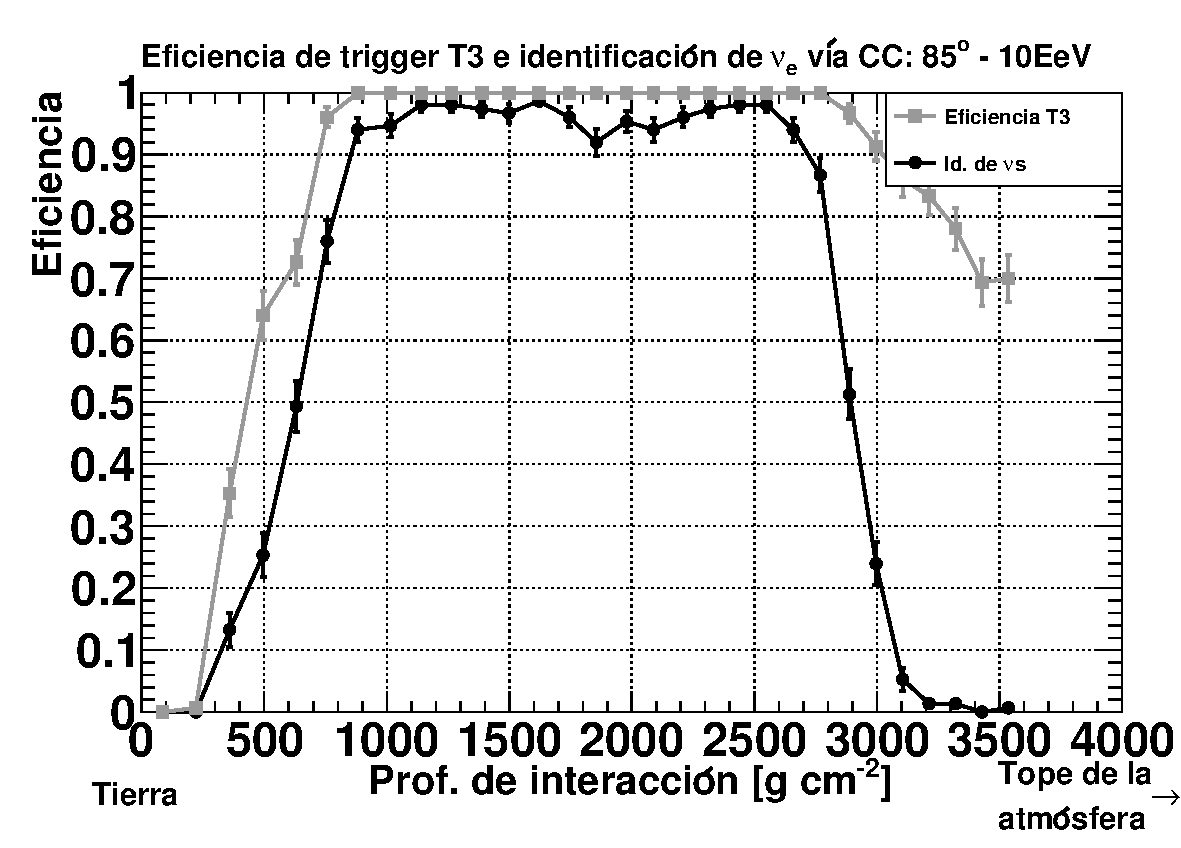
\includegraphics[width=0.7\textwidth]{fig/resultadosAuger/eff_10EeV_85}
			\caption{Eficiencia de disparo T3 e identificación en función de la profundidad de interacción para lluvias iniciadas por $\nu_e$ via CC con \cant{E_\nu=10^{19}}{eV} y \cant{\theta=85}{^\circ}}
			\label{fig:effDG_tr_id}
		\end{center}
	\end{figure} 
	%
	A esta energía y para este ángulo la eficiencia de disparo satura para profundidades intermedias.
	Cuando la lluvia se inicia muy cerca del detector no alcanza a evolucionar lateralmente lo suficiente como para disparar tres o mas estaciones, provocando menos eventos detectados. 
	Por otro lado, cuando se inicia alto en la atmósfera si bien en cerca del $70\%$ de los casos la componente muónica de la lluvia es suficiente para disparar el detector, no pueden ser identificados como neutrinos por ser muy similares a las lluvias iniciadas por hadrones.
	
	Por otro lado, en la figura \ref{fig:effDG_en} se muestran las eficiencias para lluvias iniciadas por $\nu_e$ via CC con \cant{\theta=85}{^\circ} y \cant{E_\nu=10^{17},~10^{18},~10^{19}}{eV}.
	Si bien, como era de esperarse\footnote{La cantidad de partículas que se genera con la lluvia son proporcionales a la energía de la misma.}, la eficiencia de detección disminuye con la energía del primario, las bajas energías son relativamente importantes en el cálculo de la exposición dado que los modelos actuales predicen una dependencia del tipo $E_\nu^{-2}$ para el espectro de energía de los neutrinos de origen cosmogénico.
	%
	\begin{figure}[h!]
		\begin{center}
			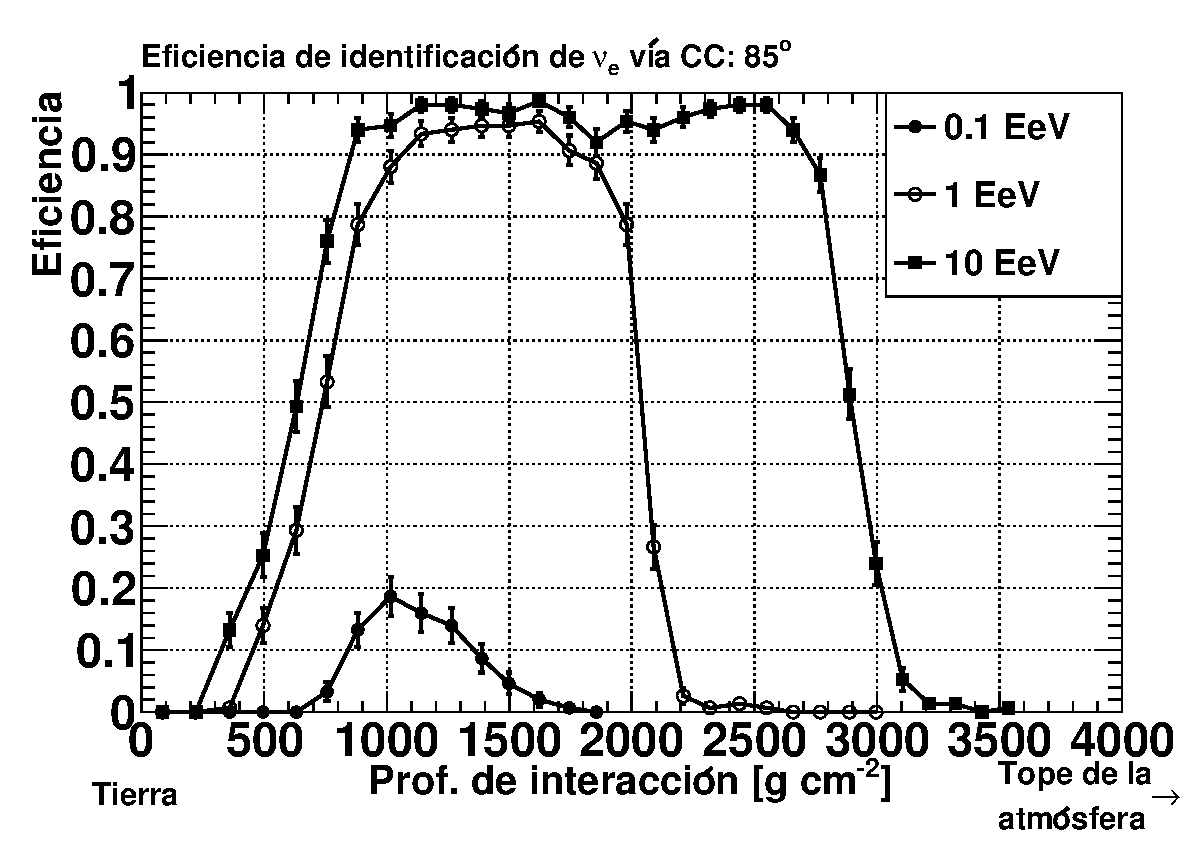
\includegraphics[width=0.7\textwidth]{fig/resultadosAuger/eff_varios_85}
			\caption{Eficiencia de identificación en función de la profundidad de interacción para lluvias iniciadas por $\nu_e$ via CC y por $\nu_x$ via CN para varias energías y \cant{\theta=85}{^\circ}}
			\label{fig:effDG_en}
		\end{center}
	\end{figure}
	%
	
	En la figura \ref{fig:effDG_th} se muestra como ejemplo las eficiencias de disparo e identificación para $\nu_e$ via CC y \cant{E_\nu=10^{18}}{eV} para \cant{\theta=80}{^\circ} en el panel izquierdo y para \cant{\theta=85}{^\circ} en el derecho.
	%
	\begin{figure}[h!]
		\begin{center}
			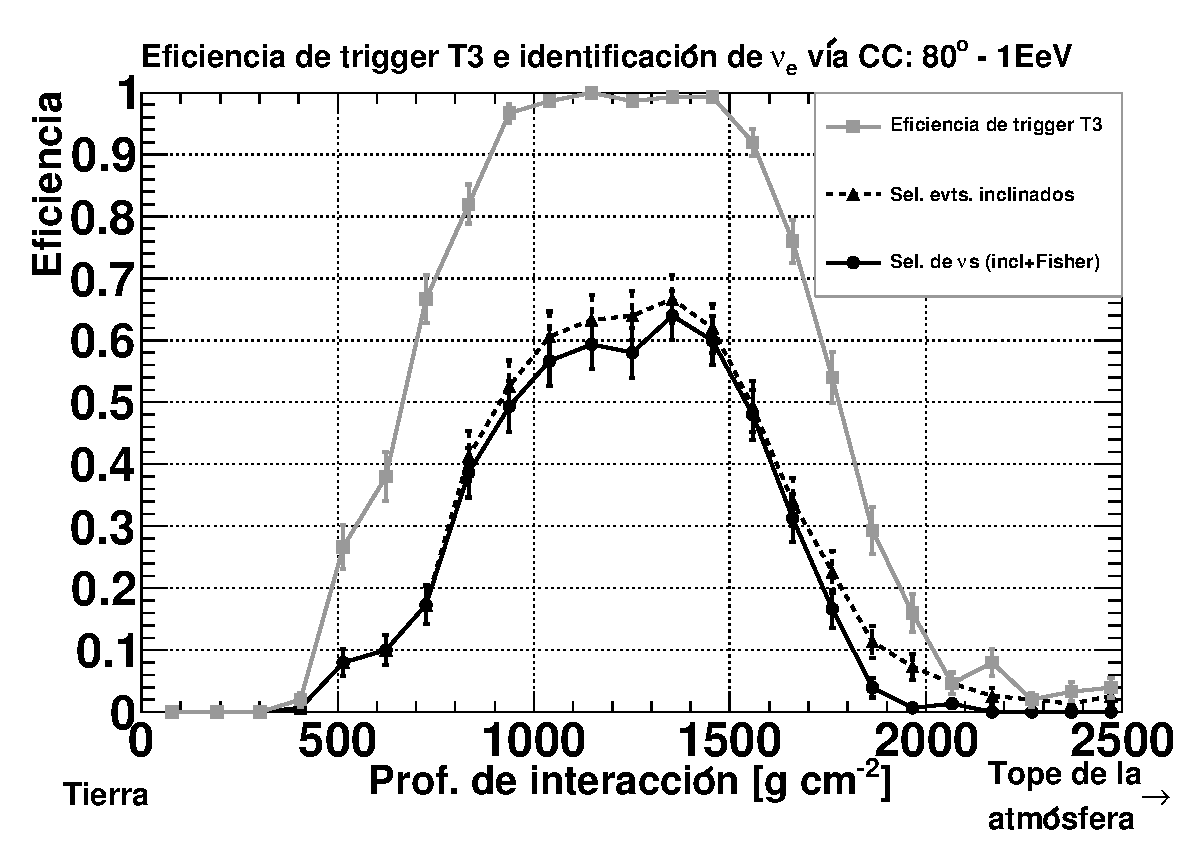
\includegraphics[width=0.47\textwidth]{fig/resultadosAuger/eff_1EeV_80}
			\hfill
			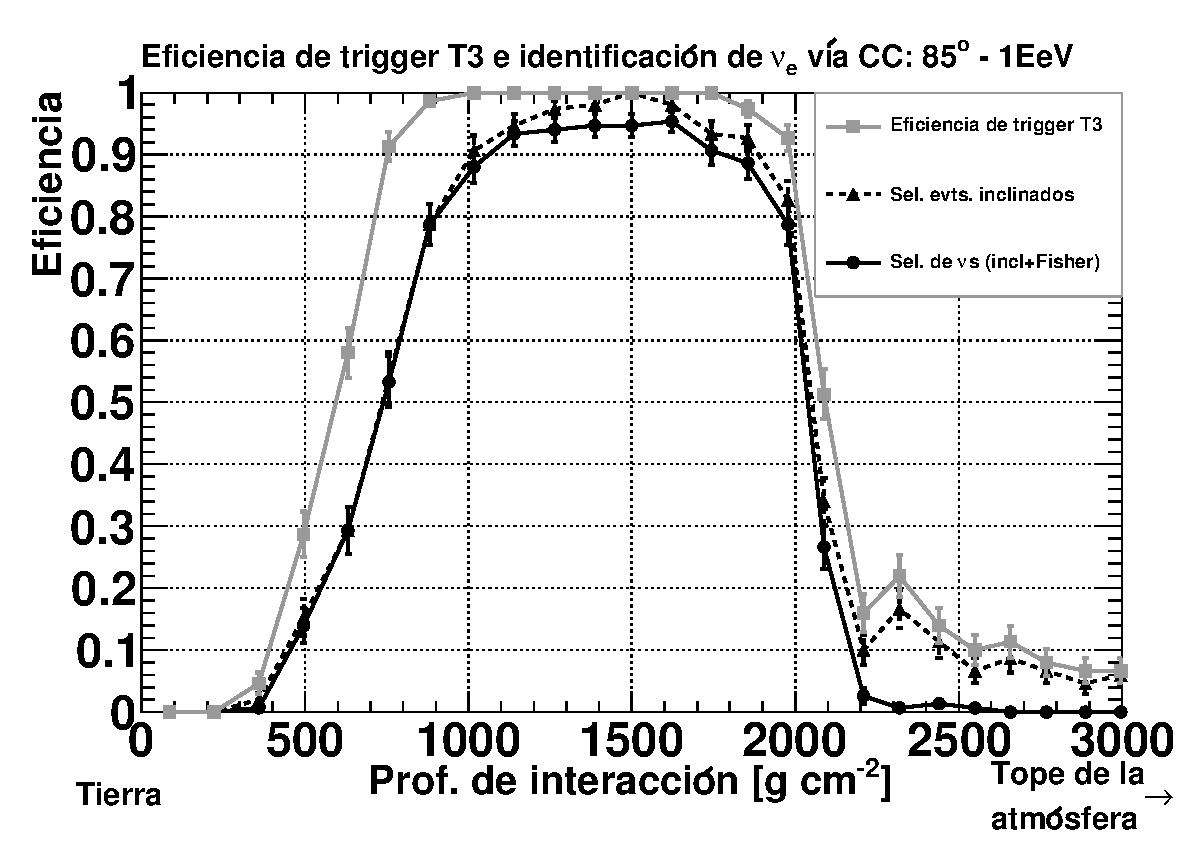
\includegraphics[width=0.47\textwidth]{fig/resultadosAuger/eff_1EeV_85}
			\caption{El panel izquierdo (derecho) muestra las eficiencias de disparo T3, de selección de eventos inclinados y de indentificación como función de la profundidad medida desde el detector para neutrinos con \cant{\theta=80}{^\circ} (\cant{\theta=85}{^\circ}). Es posible observar que la eficiencia alcanzada por el discriminante de fisher es alta para ambos ángulos.}
			\label{fig:effDG_th}
		\end{center}
	\end{figure}
	%
	En el panel izquierdo (\cant{\theta=80}{^\circ}) la eficiencia de disparo T3 alcanza el 100$\%$ a profundidades intermedias mientras que la eficiencia de identificación máxima es cercana a 60$\%$.
	Esta diferencia es producida por los cortes de selección de calidad, en los que para el canal DGH (al que corresponden estos ángulos) se requieren al menos 4 estaciones con disparo local T2, cuando el disparo global T3 requiere sólo 3.
	El panel derecho de la misma figura muestra las mismas eficiencias para \cant{\theta=85}{^\circ}, y se observa que la identificación alcanza valores cercanos a 95$\%$.
	Esta ganancia se debe a un efecto puramente geométrico, ya que la longitud de la huella sobre el detector crece con un factor aproximadamente $1/\cos\theta$, tal como se esquematiza en la figura \ref{fig:effDG_th_sktch}.
	%
	\begin{figure}[h!]
		\begin{center}
			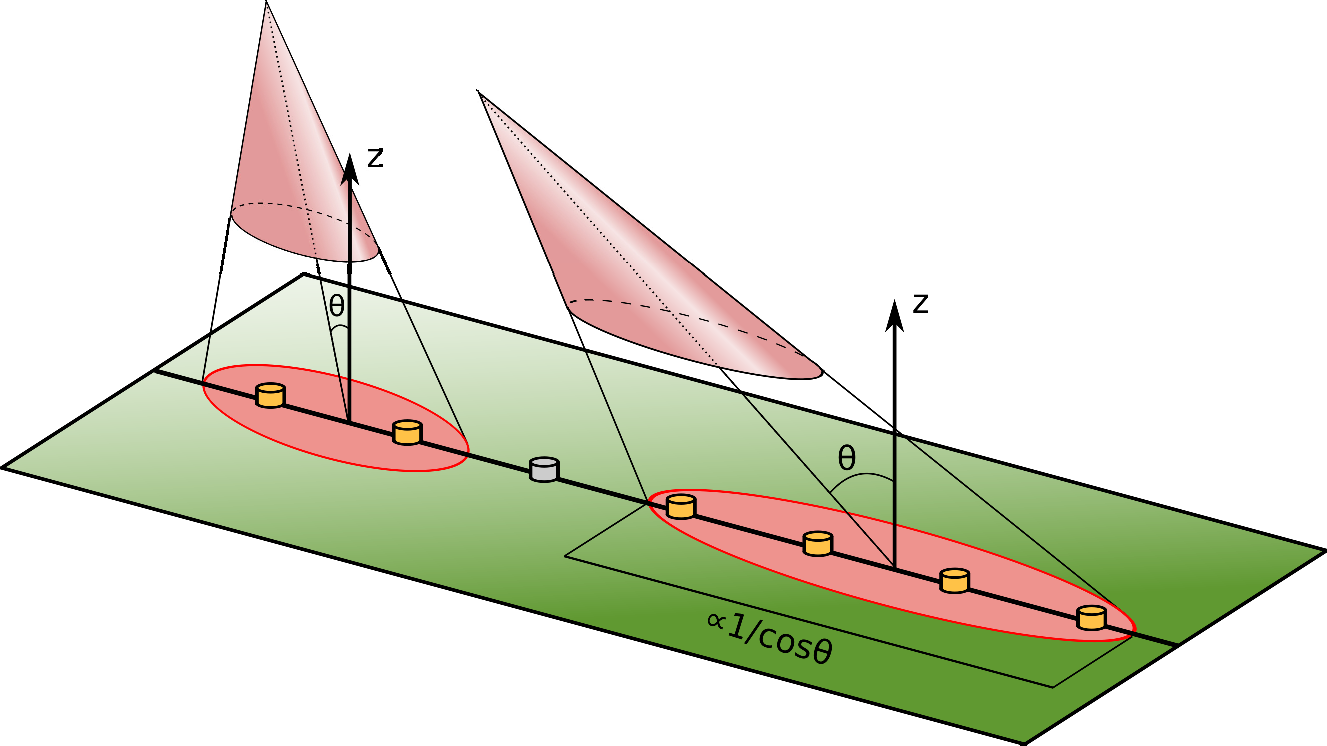
\includegraphics[width=0.7\textwidth]{fig/resultadosAuger/huellas}
			\caption{La cantidad promedio de estaciones disparadas por evento aumenta con el ángulo cenital $theta$ debido a que la huella de las llubias sobre el detector crece aproximadamente con un factor $1/\cos\theta$.}
			\label{fig:effDG_th_sktch}
		\end{center}
	\end{figure}
	%
	
	Otra particularidad de los neutrinos DG es que hay que hacer distinción entre los distintos sabores de neutrino y los canales de CC y CN.
	Dado que tanto en CN como en CC $\nu_\mu$ la energía transmitida a la lluvia es en promedio del 20$\%$ de la energía del neutrino, la eficiencia de estos canales será menor que el caso CC $\nu_e$, tal como se observa en el panel izquierdo de la figura \ref{fig:effDG_cc_nc}.
	%
	\begin{figure}[h!]
		\begin{center}
			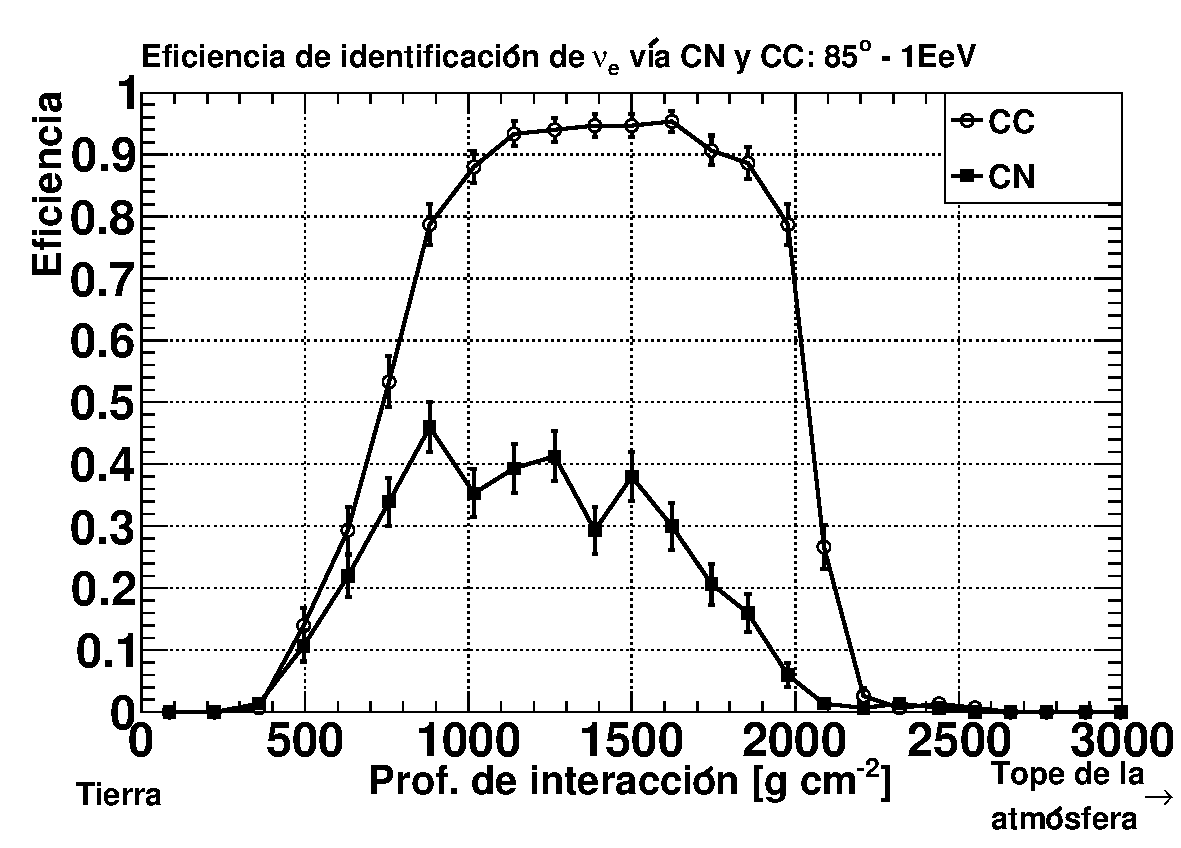
\includegraphics[width=0.47\textwidth]{fig/resultadosAuger/eff_CCvsNC_85}
			\hfill
			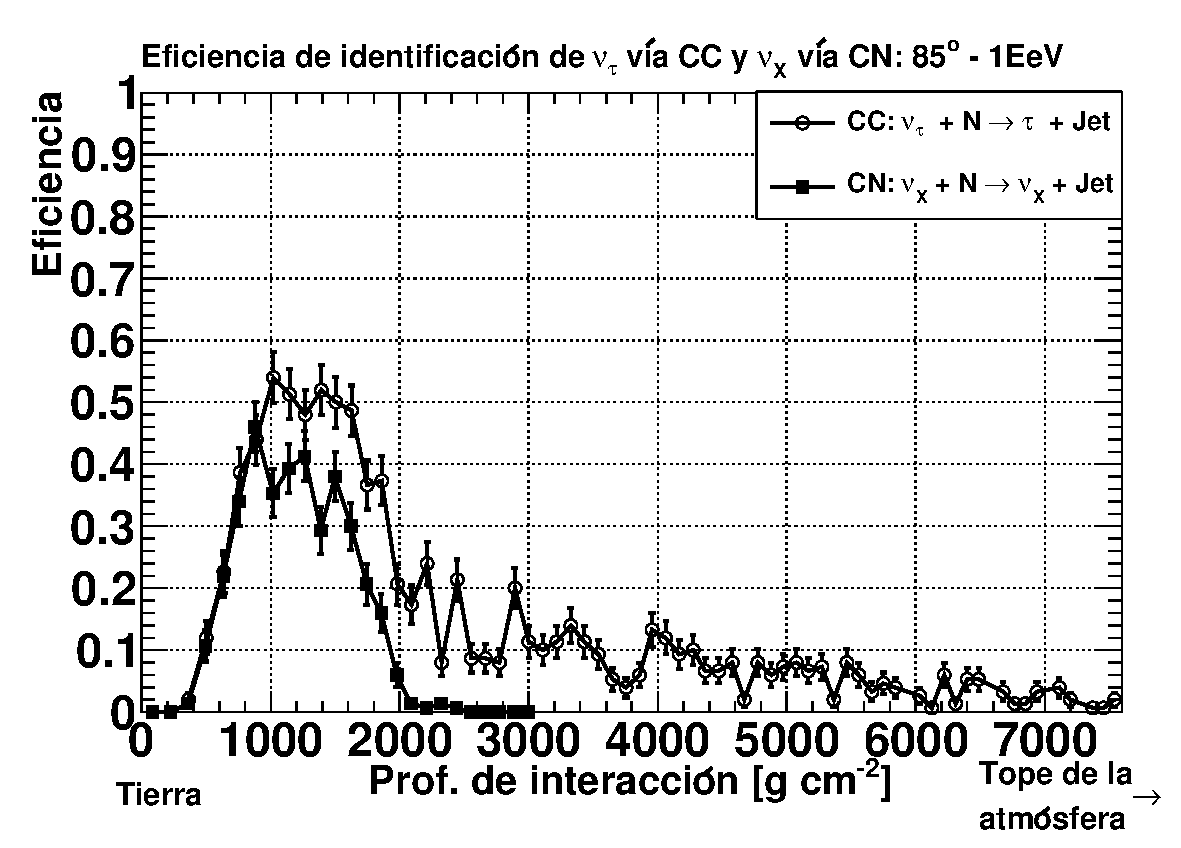
\includegraphics[width=0.47\textwidth]{fig/resultadosAuger/eff_tau_1EeV_85}
			\caption{Eficiencia de identificación en función de la profundidad de interacción para lluvias iniciadas por $\nu_e$ via CC y por $\nu_x$ via CN con \cant{10^{18}}{eV} y \cant{85}{^\circ}}
			\label{fig:effDG_cc_nc}
		\end{center}
	\end{figure}
	%
	El panel derecho de la misma se observa para los mismos parámetros la comparación entre el canal de CN y CC via $\nu_\tau$.
	En la sección \ref{sbsc:easDG} se explicó el mecanismo DB, en el que un $\nu_\tau$ interactua via CC produciendo un lepton $\tau$ que puede decaer generando una segunda lluvia a algunos km de la primer interacción.
	Teniendo en cuenta que la transferencia de energía $\nu$-nucleón no depende de si la interacción es via CC o CN, se deduce de la figura que incluso cuando la cascada generada en la primer interacción no es suficiente para disparar el detector (para profundidades mayores a \cant{\sim2000}{g cm^{-2}}) la segunda cascada a veces lo hace, recuperando del orden del 10$\%$ de los eventos.
	
	\subsubsection{Eficiencias a neutrinos ES}
	
	La eficiencia a neutrinos ES depende de los siguientes parámetros:
	%
	\begin{itemize}
	 \item la energía del tauón $E_\tau$
	 \item la altura a la que decae $x_d$
	 \item el ángulo cenital $\theta$
	\end{itemize}
	%
	En este caso, dado que tanto el canal de decaimiento del tauón y la energía acarreada por sus productos, como el ángulo azimutal $\phi$ se simularon de manera aleatorea, la eficiencia obtenida en cada bin de $(E_\tau,x_d,\theta)$ será un promedio sobre el ángulo azimutal y las maneras de decaer del tauón.
	
	En la figura \ref{fig:effES_tr_id} se muestra a modo de ejemplo la eficiencia de disparo T3 y de identificación como función de la altura de decaimiento $x_d$ para una energía de \cant{E_\tau=1}{EeV} y un ángulo cenital $\theta=90.68^\circ$.
	%
	\begin{figure}[h!]
		\begin{center}
			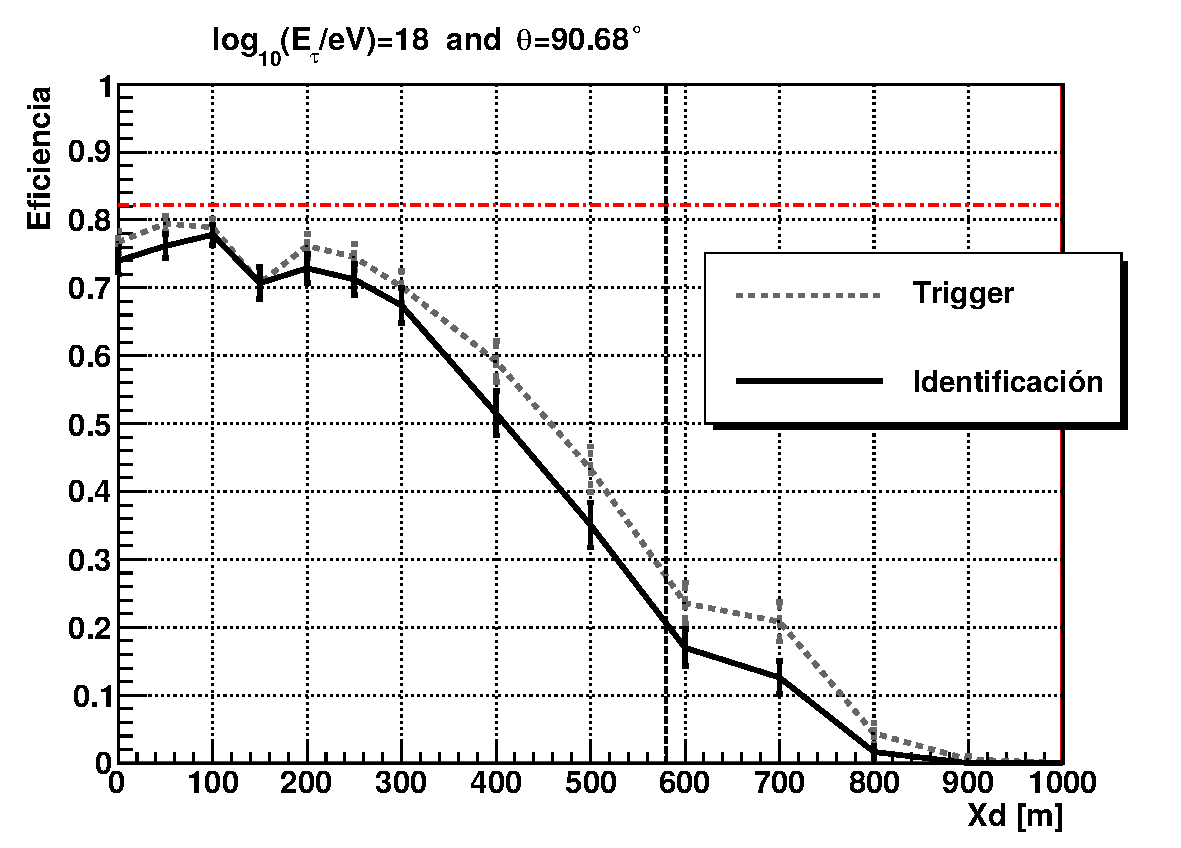
\includegraphics[width=0.7\textwidth]{fig/resultadosAuger/eff_18_8931_forThesis}
			\caption{Eficiencia de disparo T3 e identificación en función de la altura de decaimiento del tauón para \cant{E_\tau=1}{EeV} y $\theta=90.68^\circ$. La línea horizontal marca la máxima eficiencia posible debido al canal a $\mu\nu_\mu\nu_\tau$ mientras que la línea vertical señala la altura de decaimiento típica a esta energía y ángulo (ver texto).}
			\label{fig:effES_tr_id}
		\end{center}
	\end{figure}
	%
	Se observa que el criterio de identificación de neutrinos ES selecciona la mayoría de los eventos que logran disparar el detector.
	También, por debajo de \cant{x_d=300}{m} tanto la eficiencia de disparo como la de identificación alcanzan el máximo valor posile, que no puede exceder 0.822 debido a que el canal $\mu\nu_\mu\nu_\tau$ no da lluvias detectables.
	Este valor se señala con una línea horizontal punteada.
	
	Por encima de \cant{x_d=300}{m} la eficiencia decrece con $x_d$ debido a que cada vez menos partículas alcanzan el detector.
	Sin embargo, la altura característica de decaimiento para \cant{E_\tau=1}{EeV} y $\theta=90.68^\circ$ es $\lambda_h = \lambda_D\times\cos(\pi - \theta) = 4.9{\rm km} \times 0.0119 = 580{\rm m}$, como se indica con una líena punteada vertical.
	Esto quiere decir que, como se detectan eventos hasta \cant{x_d\sim800}{m}, el $75\%$ de los $\tau$'s decaerán a alturas con eficiencia de decaimiento mayor a cero.
	
	En la figura \ref{fig:effES_en} se grafica la eficiencia de identificación para \cant{E_\tau=10^{17.5},~E_\tau=10^{18},~E_\tau=10^{18.5}}{eV}.
	Como era de esperarse, existe un incremento en la eficiencia con la energía, producto de la mayor cantidad de partículas generada durante la evolución de la lluvia, que aumenta las chances de disparar más estaciones.
	%
	\begin{figure}[h!]
		\begin{center}
			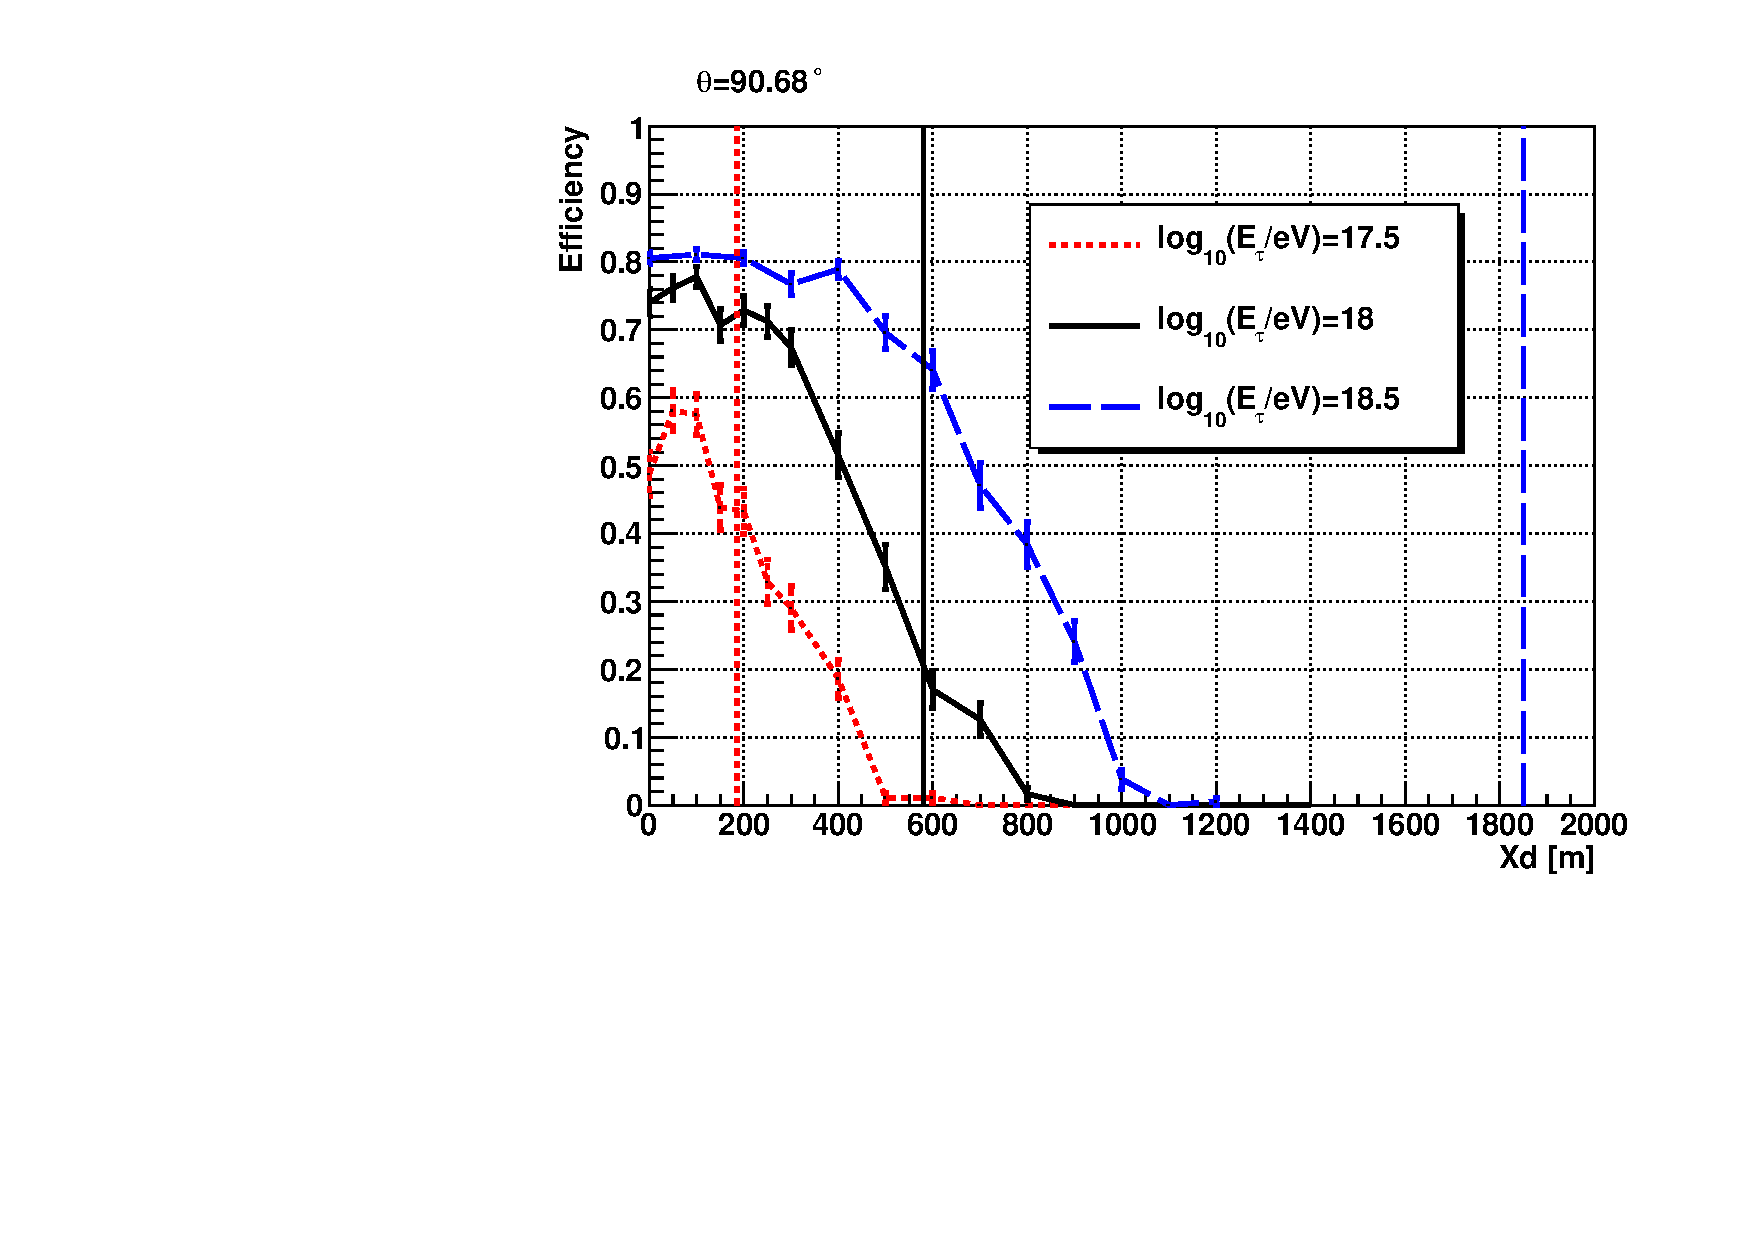
\includegraphics[width=0.7\textwidth]{fig/resultadosAuger/eff_multEnergy_forThesis}
			\caption{Eficiencia de disparo T3 e identificación en función de la altura de decaimiento del tauón para $\theta=90.68^\circ$ y diferentes energías. Las líneas verticales señalan la altura de decaimiento típica del tauón:\cant{185}{m} (\cant{E_\tau=10^{17.5}}{eV}), \cant{580}{m} (\cant{E_\tau=10^{18}}{eV}) y \cant{1850}{m} (\cant{E_\tau=10^{18.5}}{eV}).}
			\label{fig:effES_en}
		\end{center}
	\end{figure}
	%
	Por un lado, cuando el decaimiento se produce cerca del suelo (valores $x_d$ bajos) la eficiencia crece hasta alcanzar su valor máximo, 0.822.
	Por otro, a energías más altas se extiende el rango de $x_d$ con eficiencia no nula.
	Cabe destacar aunque la eficiencia crezca con la energía, la altura de decaimiento típica lo hace de manera mucho más pronunciada (directamente proporcional a la energía), por ende, en resumen, el porcentaje de eventos detectados como función de la energía decrece.
	Esto puede observarse en la figura \ref{fig:effES_en}, en la que se marca con lineas verticales la altura de decaimiento típica de cada energía. 
	
	Otro aspecto interesante de las eficiencias a neutrinos ES reside en su dependencia con el ángulo cenital.
	Como puede observarse en la figura \ref{fig:effES_th} la eficiencia decrece a medida que el tauón emerge de la tierra mas verticalmente.
	Esto se entiende debido a que las partículas del frente de la lluvia tendrán menos chances de alcanzar el suelo debido a que su dirección de propagación, en promedio, será también más vertical.
	Por otro lado, la altura de decaimiento característica del tauón depende del ángulo cenital según $\lambda_h=\lambda_D\times\cos(\pi-\theta)$, por lo que a energía fija ($\lambda_D$ fijo), la fracción de eventos detectados decrece rápidamente con el ángulo.
	Por ejemplo, para los 3 ángulos cenitales que se muestran en la figura \ref{fig:effES_th} la fracción de tauones que decaen a alturas en las que la eficiencia de identificación es 0 es 0.21 a $\theta=90.68^\circ$, 0.68 a $\theta=91.83^\circ$ y 0.85 a $\theta=92.98^\circ$.
	%
	\begin{figure}[h!]
		\begin{center}
			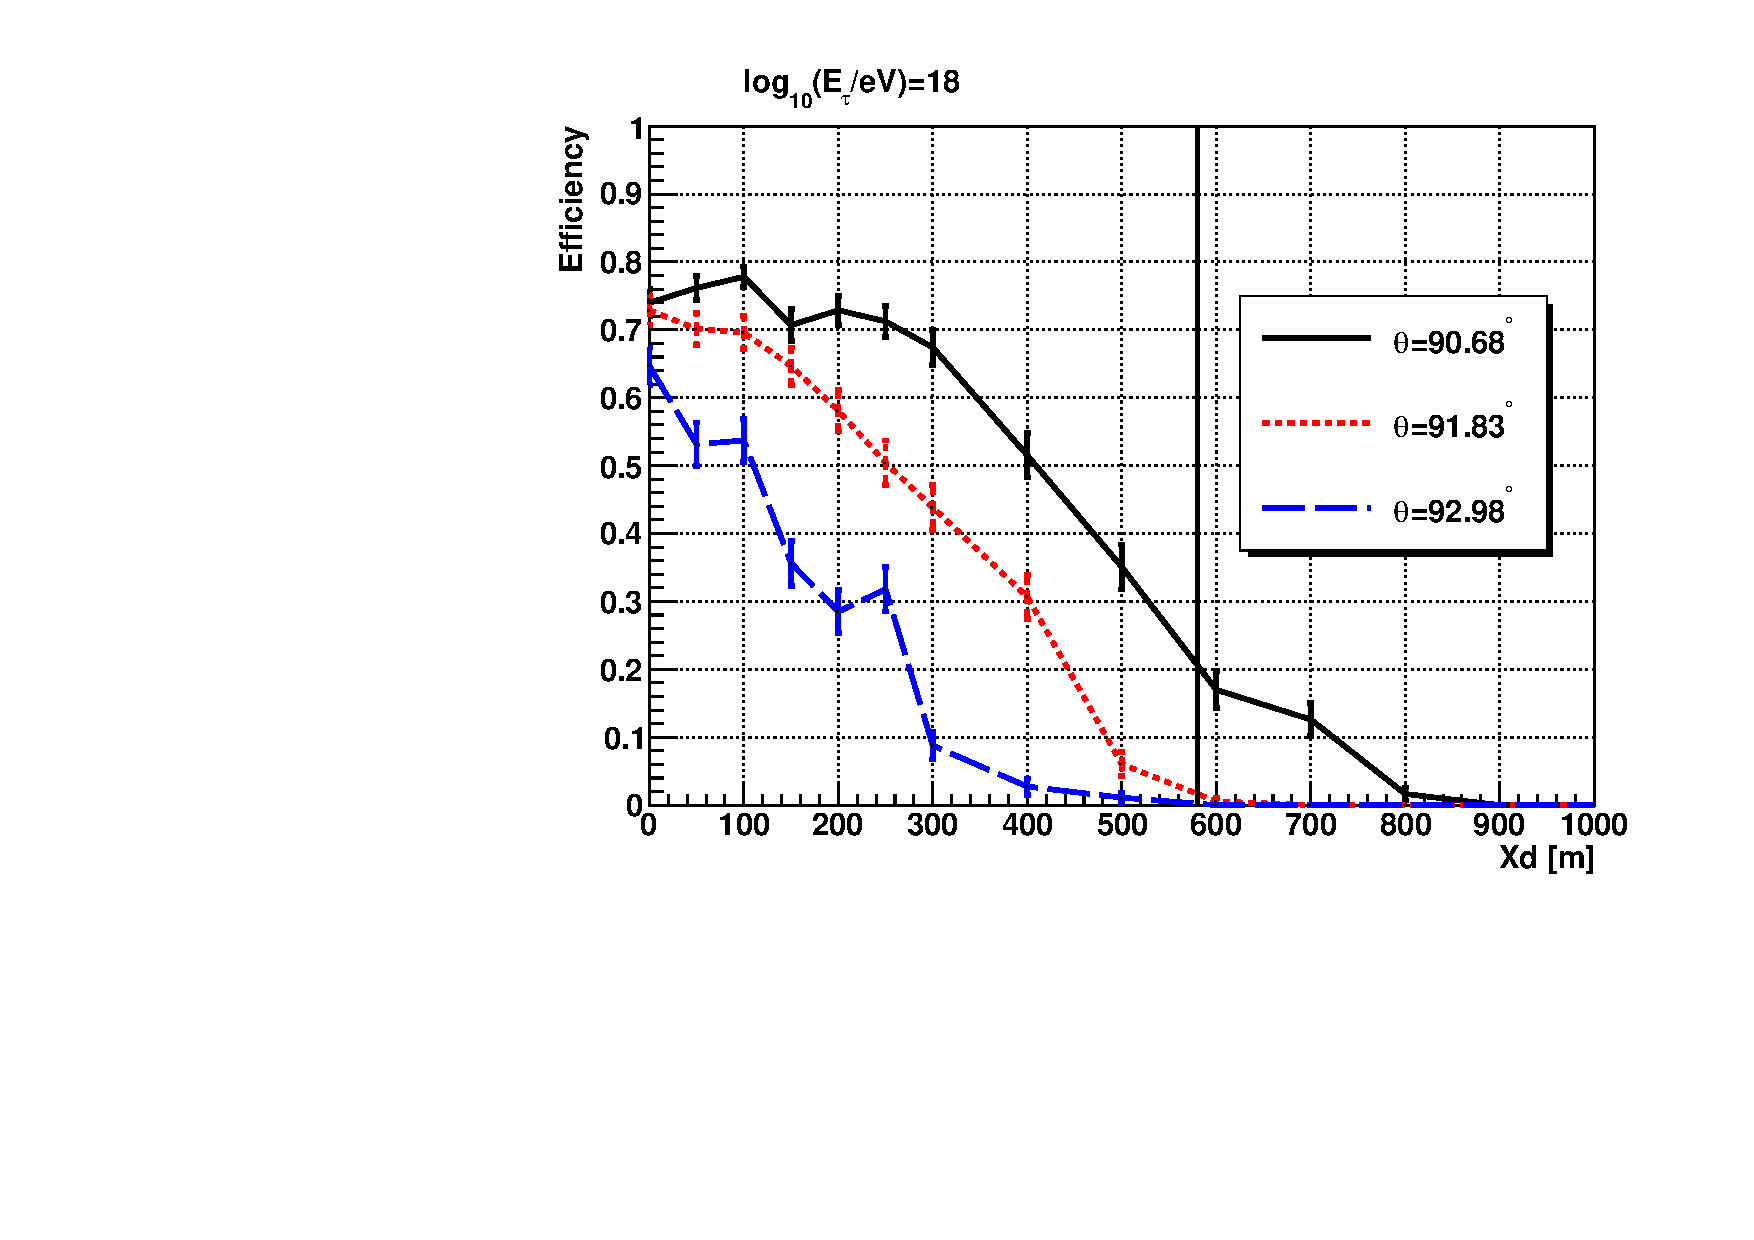
\includegraphics[width=0.47\textwidth]{fig/resultadosAuger/eff_multiTheta_forThesis}
			\hfill
			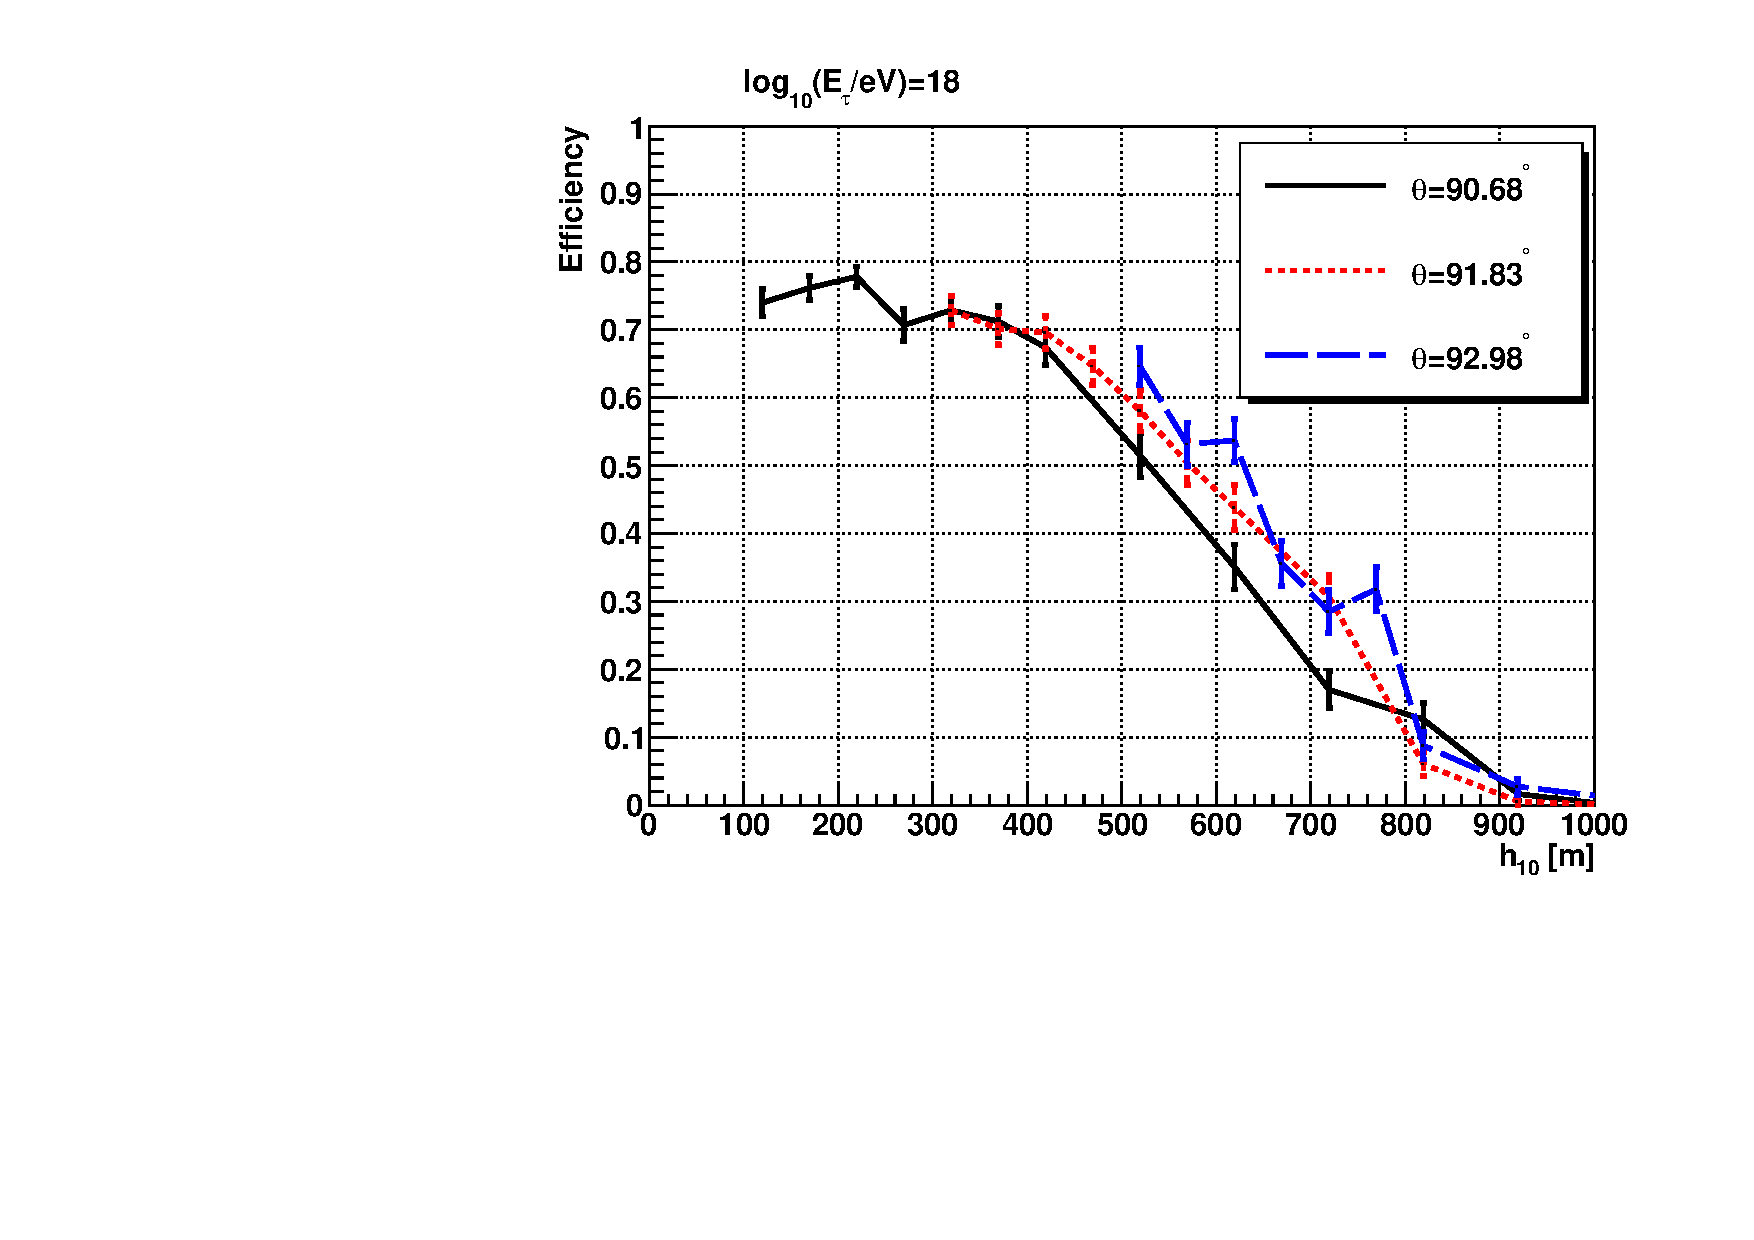
\includegraphics[width=0.47\textwidth]{fig/resultadosAuger/eff_multTheta_h10_forThesis}
			\caption{Izquierda: eficiencia de identificación como función de la altura de decaimiento del tauón con energía \cant{E_\tau=10^{18}}{eV} y varios ángulos cenitales. La líena vertical a \cant{x_d=580}{m} marca la altura típica del decaimiento para $\theta=90.68^\circ$. Para $\theta=91.83^\circ$ y $\theta=92.98^\circ$ las alturas típicas de decaimiento son 1560 y \cant{2540}{m}, fuera de escala.
			Derecha: Las mismas eficiencias pero como función del parámetro $h_{10}$ (ver texto).}
			\label{fig:effES_th}
		\end{center}
	\end{figure}
	%
	
	Es muy interesante introducir la variable $h_10\equiv x_d + 10{\rm km} \times\cos(\pi-\theta)$, que corresponde a la altitud del eje de la lluvia a \cant{10}{km} del decaimiento del tauón.
	En el panel derecho de la figura \ref{fig:effES_th} se uestra la eficiencia como función de $h_{10}$ para los 3 ángulos cenitales.
	Puede observarse como a primer orden, la eficiencia de identificación no depende de $\theta$ y $x_d$ por separado sino de $h_{10}$.
	Esto se debe a que al tratarse de eventos muy horizontales, la probabilidad de detección depende básicamente de la altura a la que se alcanza el máximo desarrollo de la lluvia \cite{verTesisYann125}.
	Para las energías consideradas en este análisis, este máximo se produce aproximadamente a \cant{10}{km} del decaimiento del tauón.
	En particular, la figura \ref{fig:effES_th} muestra que es altamente improbable detectar un evento iniciado por un tauón de \cant{E_\tau=10^{18}}{eV} cuyo máximo se produce a más de \cant{1000}{m} sobre detector.
	 
	
	\subsection{Integración de las eficiencias sobre el área del detector}
	
	Para llevar a cabo la integración en área de la ecuación \ref{eq:exp2} es necesario estudiar cómo varían las eficiencias cuando se considera un detector finito, es decir, con bordes.
	Cuando una lluvia cae sobre una región completamente instrumentada del detector (interior y sin estaciones faltantes) la eficiencia será la ideal, calculada en la sección \ref{sbsc:idealEff}.
	Sin embargo, existen casos en los que el baricentro de las partículas de la lluvia puede caer hasta una decena de kilómetros fuera del detector y aun así disparar suficientes estaciones para ser identificado como neutrino. 
	Esto se esquematiza en la figura \ref{fig:lluviaFuera} para neutrinos DG y ES.
	%
	\begin{figure}[h!]
		\begin{center}
			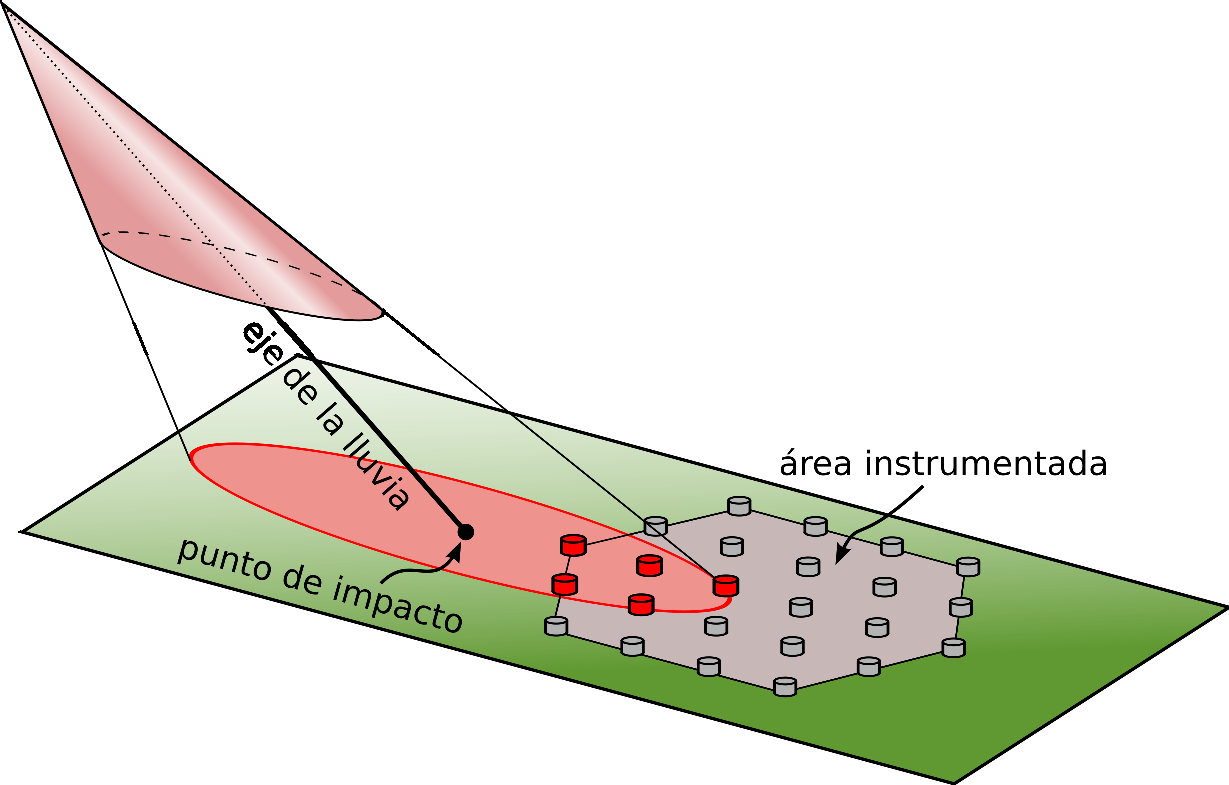
\includegraphics[width=0.8\textwidth]{fig/resultadosAuger/lluviaFuera}\\
			\vspace*{0.1\textwidth}
			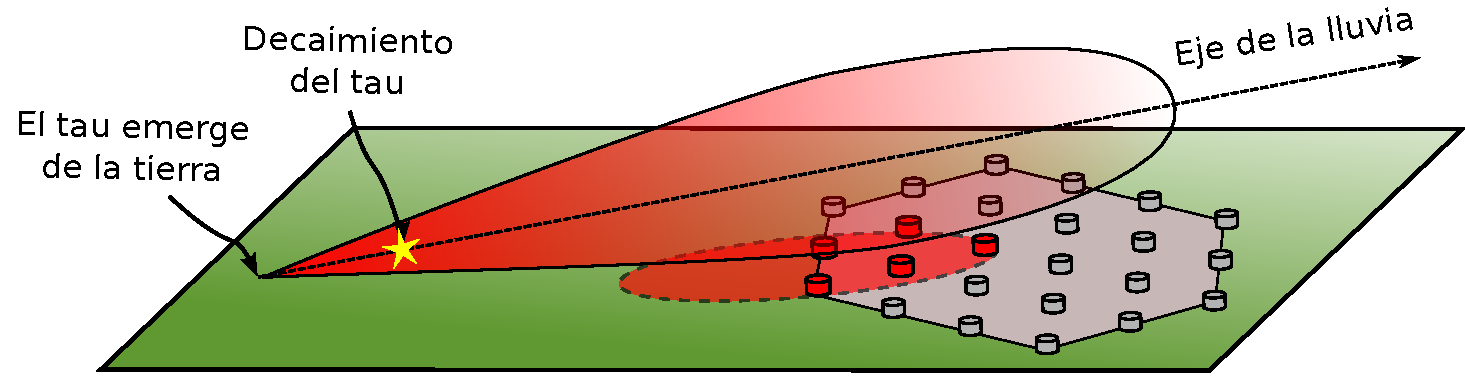
\includegraphics[width=0.8\textwidth]{fig/resultadosAuger/lluviaFuera_ES}
			\caption{asd}
			\label{fig:lluviaFuera}
		\end{center}
	\end{figure}
	%
	
	En este contexto, se define un área circular extendida que contiene al detector finito y es suficientemente grande como para contemplar la contribución de las lluvias cuyo punto de impacto $\vec{r}$ cae fuera del detector\footnote{En otras palabras, el tamaño del círculo se selecciona tal que las lluvias que caen fuera de él tiengan un probabilidad nula de disparar el detector.} (ver figura \ref{fig:aperturaReal}).
	
	Realizar la integral en área de la eficiencia consiste en hallar la eficiencia de identificación promedio en el área circular extendida~$A$.
	%
	\begin{equation}
	\langle\epsilon(\psi)\rangle_{\rm A} \equiv \epsilon(\psi) =
	\frac{\int\!\epsilon(\vec{r},\psi)\,{\rm d}A}{A}
	\end{equation}
	%
	En esta ecuación, $\psi$ representa los parámetros $(E_\nu,\theta,D)$ para el canal DG y $(E_\tau,\theta,x_d)$ en ES.
	Esta eficiencia depende de la cantidad y distribución espacial (configuración) de las estaciones de superficie que conforman al detector finito que se está considerando.
	Es importante notar que si bien $\epsilon(\psi)$ depende de la elección del área extendida $A$ (cae al aumentarla), su producto $\epsilon(\psi)\times A$ es una constante que define una propiedad intrínseca del detector llamada área efectiva $A_{\rm ef}$:
	%
	\begin{equation}
	A_{\rm ef}(\psi,t)=\int\!\epsilon(\vec{r},\psi,t)\,{\rm d}A
	\label{eq:Aeff}
	\end{equation}
	%
	Este área representa la superficie de un detector equivalente 100\% eficiente.
	Para calcular esta magnitud, se podría en principio, repetir para cada configuración, la cadena de simulación completa desde la generación de la primera interacción a la respuesta del detector (finito en este caso).
	Sin embargo, este camino es impráctico y requeriría un volumen de cómputo inaceptable.
	Por esta razón, se decidió tomar un enfoque diferente en el que fuera posible reusar las simulaciones producidas sobre el detector infinito para calcular la eficiencia de identificación de todas las posibles configuraciones del SD real.

	Los puntos de impacto $\vec{r}$ de las lluvias simuladas sobre un arreglo ideal son ubicados al azar dentro de la circunferencia del área extendida y las estaciones de los eventos simulados sobre el arreglo infinito que no coinciden con una estación activa del arreglo finito son descartadas (ver figura \ref{fig:aperturaReal}).
	De esta manera se calcula el evento que se obtendría si la simulación se hubiera realizado sobre el detector finito.
	Utilizando las estaciones así seleccionadas, se reevalúan las condiciones de trigger T3 y, en caso de que se satisfagan, se recomputan las variables globales, los cortes de selección de lluvias inclinadas y lluvias jóvenes. 
	En la figura \ref{fig:aperturaReal} se resume, a modo de ejemplo, los resultados posibles de reevaluar un evento que se identifica como neutrino sobre un arreglo infinito.
	
% 	El cociente de eventos identificados sobre eventos totales, determina la eficiencia de identificación promedio $\epsilon(E_\nu,\theta,D)$ de la configuración:
% %
% \begin{equation}
% \epsilon (E_\nu, \theta, D) = \frac{N_{\rm id}(E_\nu, \theta, D)}{N_{\rm sim}(E_\nu, \theta, D)} 
% \end{equation}
% %
% El $A_{\rm ef}(E_\nu,\theta,D,t)$ se obtiene multiplicando este valor por la superficie del área extendida $A$.
	
	%
	\begin{figure}[h!]
		\begin{center}
			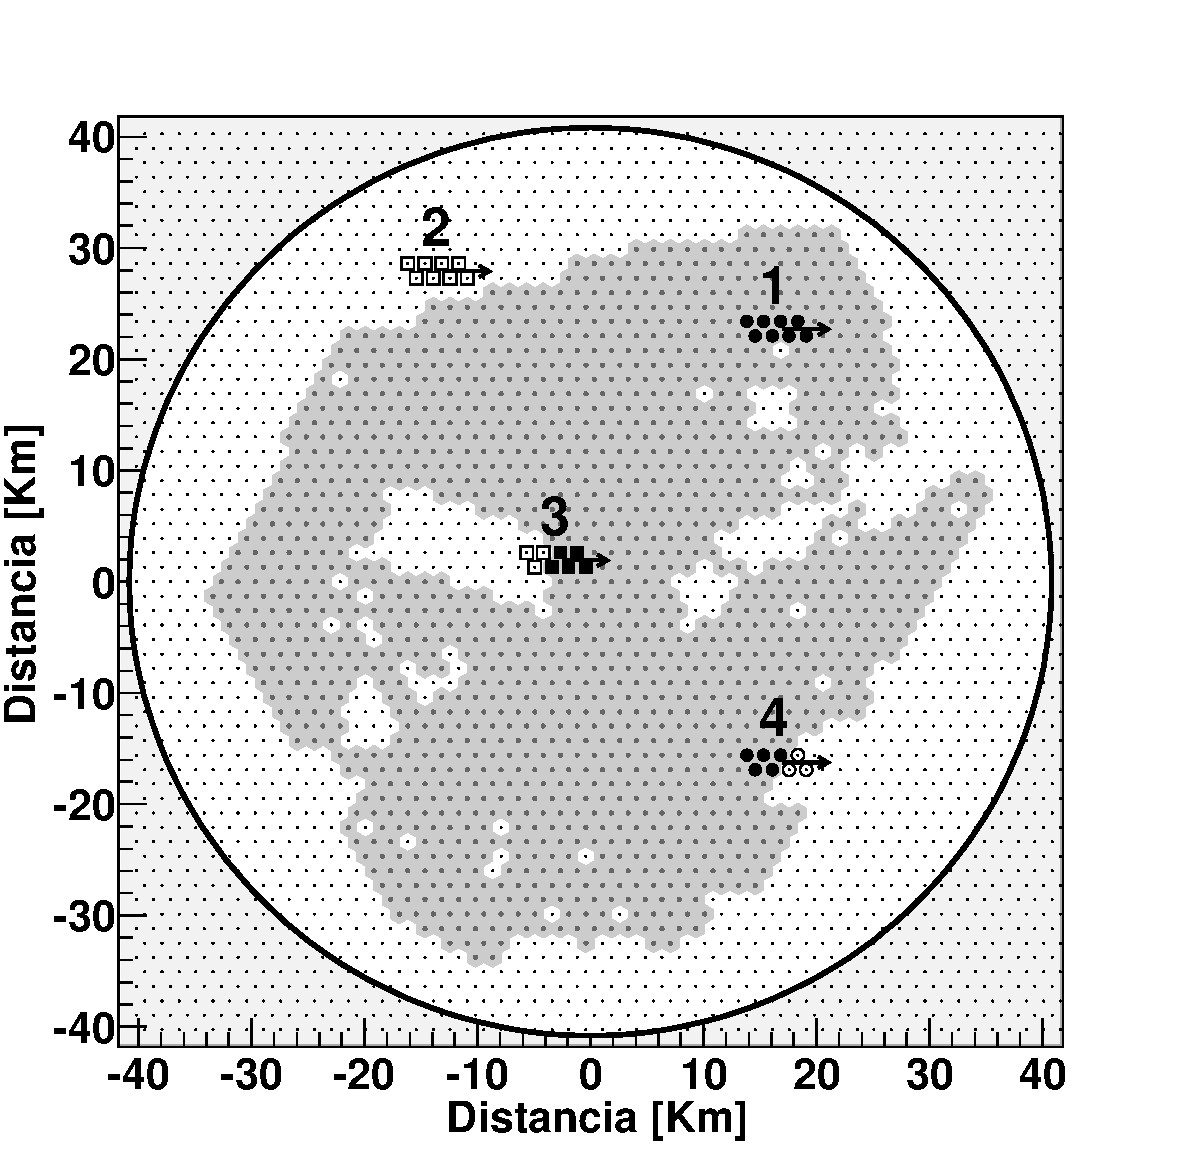
\includegraphics[width=0.63\textwidth]{fig/resultadosAuger/aperturaReal}
			\caption{Ejemplo del resultado de ubicar la misma lluvia, iniciada por un neutrino profundo, en cuatro posiciones diferentes, sobre una configuración dada del detector.
			Las flechas indican la dirección de avance de la lluvia, los puntos representan el arreglo ideal e infinito de estaciones y la circunferencia el área de detección extendida (ver texto).
			Los símbolos sólidos corresponden a estaciones de la lluvia simulada que presentan trigger T2 y que también están activas en la configuración de referencia.
			Los símbolos abiertos indican estaciones que no se encuentran en el arreglo real. Los símbolos redondos indican las lluvias identificadas como neutrinos y los cuadrados las que no.
			En el caso~1 la lluvia está completamente contenida y es identificada como neutrino. En~2 cae completamente fuera de la configuración de referencia y, por lo tanto, no produce T3 sobre el detector real.
			Aunque en el caso~3 la lluvia está parcialmente contenida y dispara el SD, no es identificada como neutrino debido a que sus estaciones tempranas no son registradas en el detector real. En~4, la lluvia pierde sus estaciones tardías pero es aún identificada ya que conserva su región temprana que es la que más influye en la discriminación.}
			\label{fig:aperturaReal}
		\end{center}
	\end{figure}
	%
% 	\clearpage
	
	\subsection{Integración temporal: evolución del detector}
	
	Incluir la evolución temporal del detector en la integración de la ecuación \ref{eq:exp2} no es simple.
	Si bien la construcción del SD de Auger concluyó a finales de 2008, y se comporta de manera estable desde entonces, es común que algunas estaciones entren o salgan de servicio por mantenimiento, fallas o situaciones fortuitas.
	Por este motivo el estado del detector es monitoreado cada segundo mediante la frecuencia de disparo T2 de todas las estaciones.
	A partir de esta información se generan archivos que registran las configuraciones (conjunto de estaciones activas) del SD con una resolución de un segundo.
	
	Entonces, de manera ideal, habría que evaluar la exposición de todas las configuraciones por las que pasa el detector y realizar la integración mediante una suma pesada por la cantidad de tiempo que se mantiene en cada una.
	Como no es posible procesat tal cantidad de información, se dividió el periodo de búsqueda de en intervalos de 3 días y se tomó, para cada uno de ellos, una configuración de representativa. 
	Luego, a cada una de estas configuraciones se le asignó un peso determinado por la fracción del tiempo en que el detector se encuetra en dicha configuración representativa, o en una de mayor eficiencia dentro de dicho intervalo.
	
	Para cada periodo de tiempo, no es evidente cual de las configuraciones por las que pasa el SD es conveniente elegir.
	Para abordar este problema se trabajó bajo la aproximación de que, dentro de los 3 días de duración del periodo, la exposición es una función de la cantidad de estaciones activas y no de su distribución espacial particular.
	Si bien es claro que esta aproximación no es válida en general\footnote{Por ejemplo, a misma cantidad de estaciones, una fila de estaciones no tiene la misma exposición que un arreglo cuadrado}, es muy buena al restringirse a periodos de tiempo lo suficientemente cortos tal que las configuraciones, con muchas estaciones activas, por las que pasa el detector son muy similares.
	
	En la figura \ref{fig:t2FilePlot} se muestra, a modo de ejemplo, la cantidad de estaciones activas en función del tiempo para el periodo que va del 3/01/08 al 5/01/08. Las zonas sombreadas corresponden a periodos, conocidos como ``bad periods", en los que el detector se encontraba particularmente inestable y que son removidos del análisis.
	Como puede verse, la cantidad de estaciones activas es esencialmente constante la mayor parte del tiempo con la excepción de breves periodos en los que puede caer significativamente.
	En estos intervalos la configuración espacial del detector puede ser significativamente diferente y la aproximación de que la exposición depende solo del número de estaciones deja de ser válida.
	Es por ello que estos intervalos son eliminados y se restan de la fracción de tiempo en que se considera activa a la configuración de referencia, es decir, se subestima la eficiencia como 0.
	
	Para elegir la confguración de referencia se busca maximizar el producto $N \times F$, en donde $N$ es la cantidad de estaciones activas y $F$ la fracción de tiempo que el detector permanece en la configuración de referencia o en una equivalente (esto es, con igual o mayor número de estaciones activas).
	Entonces, con este criterio se selecciona una configuración representativa para cada uno de los periodos de 3 días.
	Si para un periodo existe más de una configuración, se toma la que ocurre primero en el tiempo (es indistinto bajo la aproximación en que se trabaja).
	Este método permite obtener una cota inferior para la exposición del detector, ya que siempre se subestima la cantidad de tiempo que este permanece activo.
	Con el fin de estimar este error sistemático se estudió, para un intervalo de tiempo reducido, como varía la exposición al considerar periodos de duración inferior a los 3 días. Se obtuvo como resultado que la diferencia es del orden del 1\%, muy por debajo de las otras fuentes de error que se discuten en la sección \ref{sc:systErr}.
	%
	\begin{figure}[ht!]
	\begin{center}
	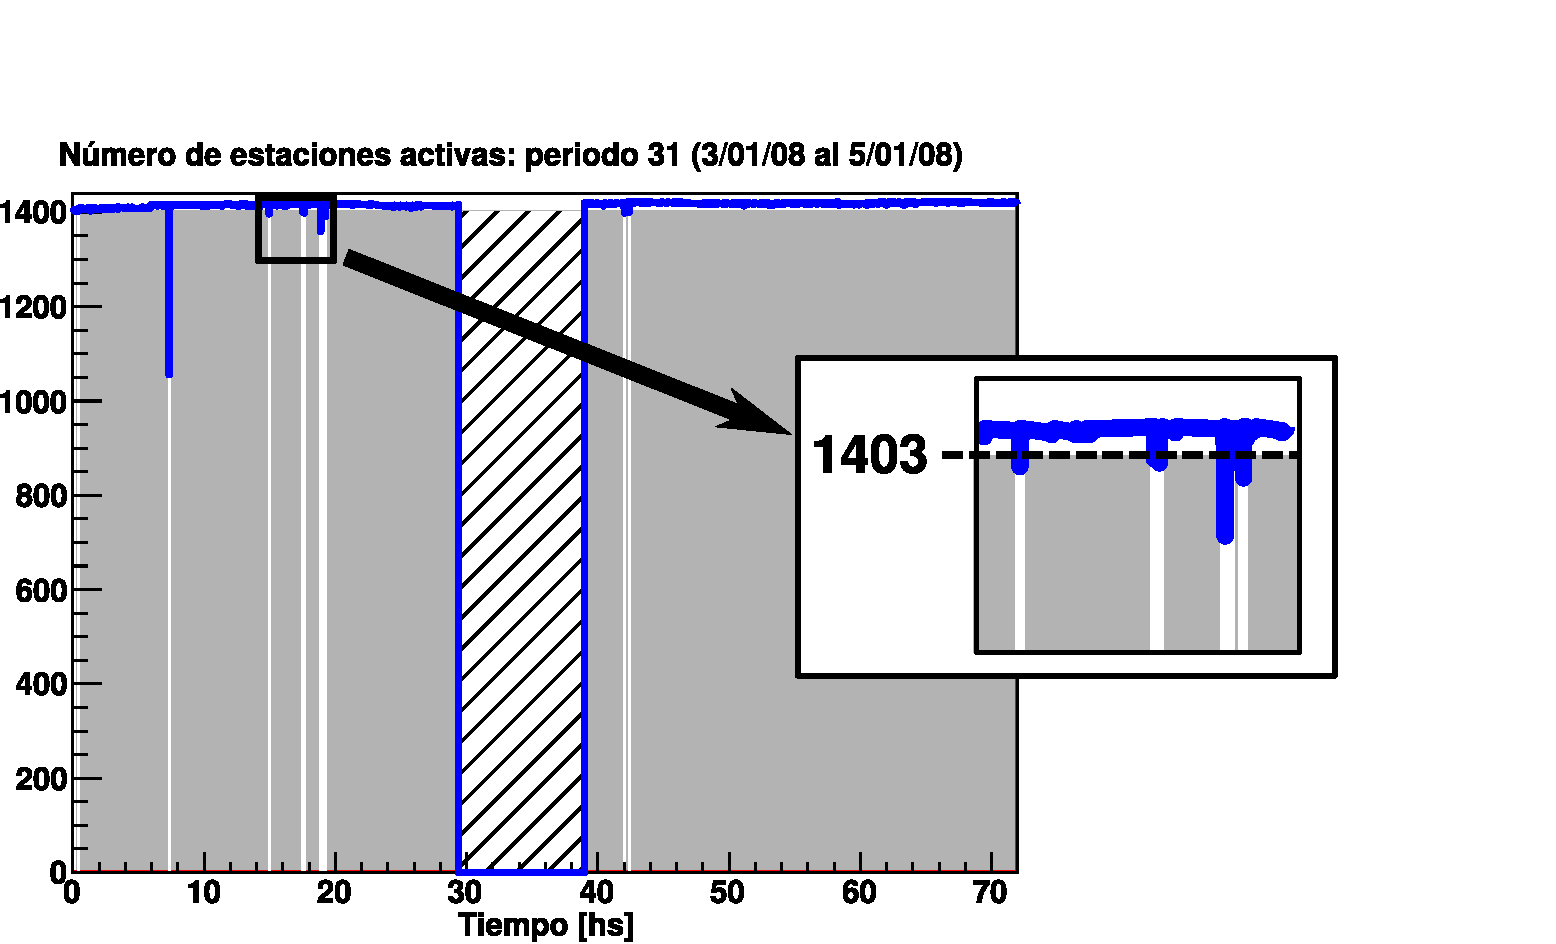
\includegraphics [width=0.90\textwidth]{fig/resultadosAuger/t2FilePlot.pdf}
	\caption{Cantidad de estaciones activas en función del tiempo para el periodo periodo del 3/01/08 al 5/01/08. La zona tachada corresponden a un ``bad period" (ver texto). La configuración de referencia elegida para este periodo cuenta con 1403 estaciones activas.
	La zona sombreada corresponde a $N \times T$ en donde $N$ es la cantidad de estaciones activas y $T$ el tiempo en que el detector permanece en la configuración de referencia o en una equivalente (esto es, con igual o mayor número de estaciones activas).}
	\label{fig:t2FilePlot}
	\end{center}
	\end{figure}
	%
	
	\subsubsection{Envejecimiento del detector}
	
	Además de la cantidad de estaciones activas, otro factor a tener en cuenta a la hora de realizar la integración temporal es el envejecimiento del detector.
	Para ello, es necesario contemplar cómo se modifica con el paso del tiempo el comportamiento de sus distintos componentes, sobre todo cuando éste afecta la señal registrada.
	
	Ante el pasaje de partículas por la estación, la señal en el PMT presenta un flanco de subida abrupto y un decaimiento exponencial.
	Mientras que el rápido crecimiento inicial se encuentra dominado por una única reflexión de la luz Cherenkov en el Tyvec de la estación, el decaimiento posterior se produce debido a varias de estas reflexiones.
	Es por esto que tanto la reflectividad del Tyvec como la longitud de absorción de la luz en el agua son parámetros de la estación que afectan fuertemente las características de la señal.
	Por otro lado, por ejemplo debido a que las estaciones se encuentran a al intemperie\footnote{Las estaciones sufren cambios de temperatura diarios, estacionales y hasta episodios de congelamiento.}, ambos parámetros son afectados por el envejecimiento del detector y habrá que tener en cuenta su variación a la hora de simular las estaciones.
	
	Si bien hasta la fecha no existe ningún mecanismo implementado que permita monitorear constantemente la reflectividad del Tyvec (TyRef) y la absorción del agua (wAbs) de las estaciones, el tiempo de decaimiento de la señal (LDT por sus siglas en inglés, \emph{light decay time}) depende fuertemente de estos parámetros y sirve como una medida indirecta de los mismos.
	Entonces, para modelar el detector se estudiará el comportamiento de esta cantidad en función del tiempo, y además su dependencia con los parámetros TyRef y wAbs.
	
	Con esto en mente, la estrategia es la siguiente:
	\begin{enumerate}
	 \item \textbf{Estudiar el LDT:} para entender la evolución del detector es importante estudiar el comportamiento del LDT en los distintos sectores del detector como función del tiempo.
	 \item \textbf{Definir una estrategia de simulación:} teniendo en cuenta cuánto y cómo varía el LDT es posible decidir cómo se modelará el detector. Esto puede implicar utilizar un detector promedio o incluso uno que incluya sus fluctuaciones segun el momento y la posición de la estación.
	 \item \textbf{Obtener LDT(tyRef,wAbs):} dado que para simular la señal en las estaciones con \Offline{} se utilizan como parámetros de entrada la reflectividad del Tyvec y la absorción del agua, será necesario analizar como obtener el valor de LDT buscado como función de estos parámetros.
	\end{enumerate}

	En la figura \ref{fig:ldtArray} se muestra como ejemplo la distribución de LDT promedio de cada estación del array en el mes de Enero de 2005, 2008 y 2013. 
	%
	\begin{figure}[ht!]
		\begin{center}
			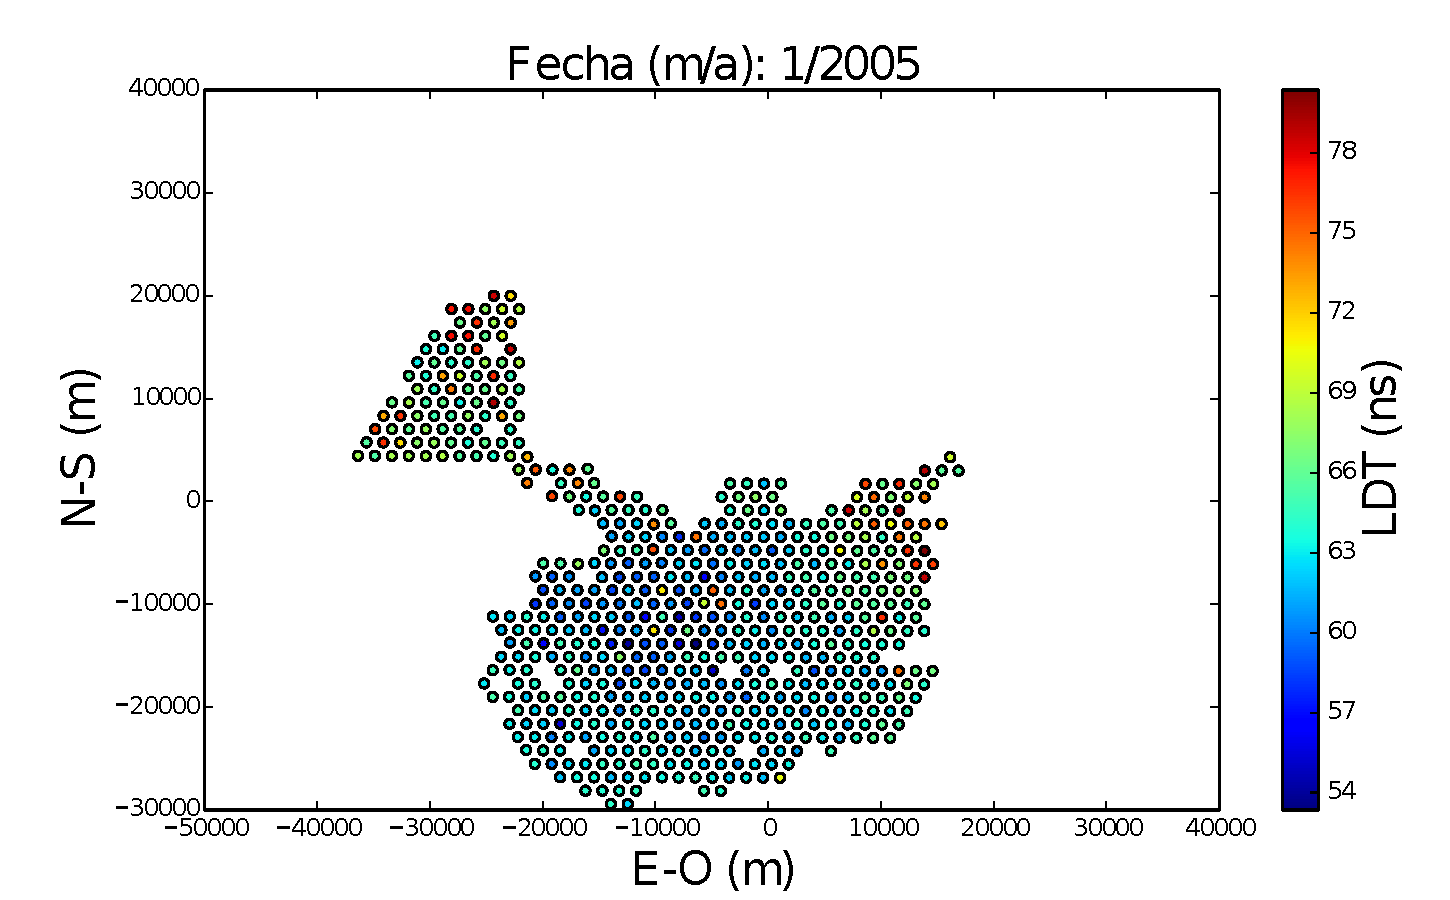
\includegraphics[width=0.67\textwidth]{fig/resultadosAuger/Out_decaytime_main_2005_01}
			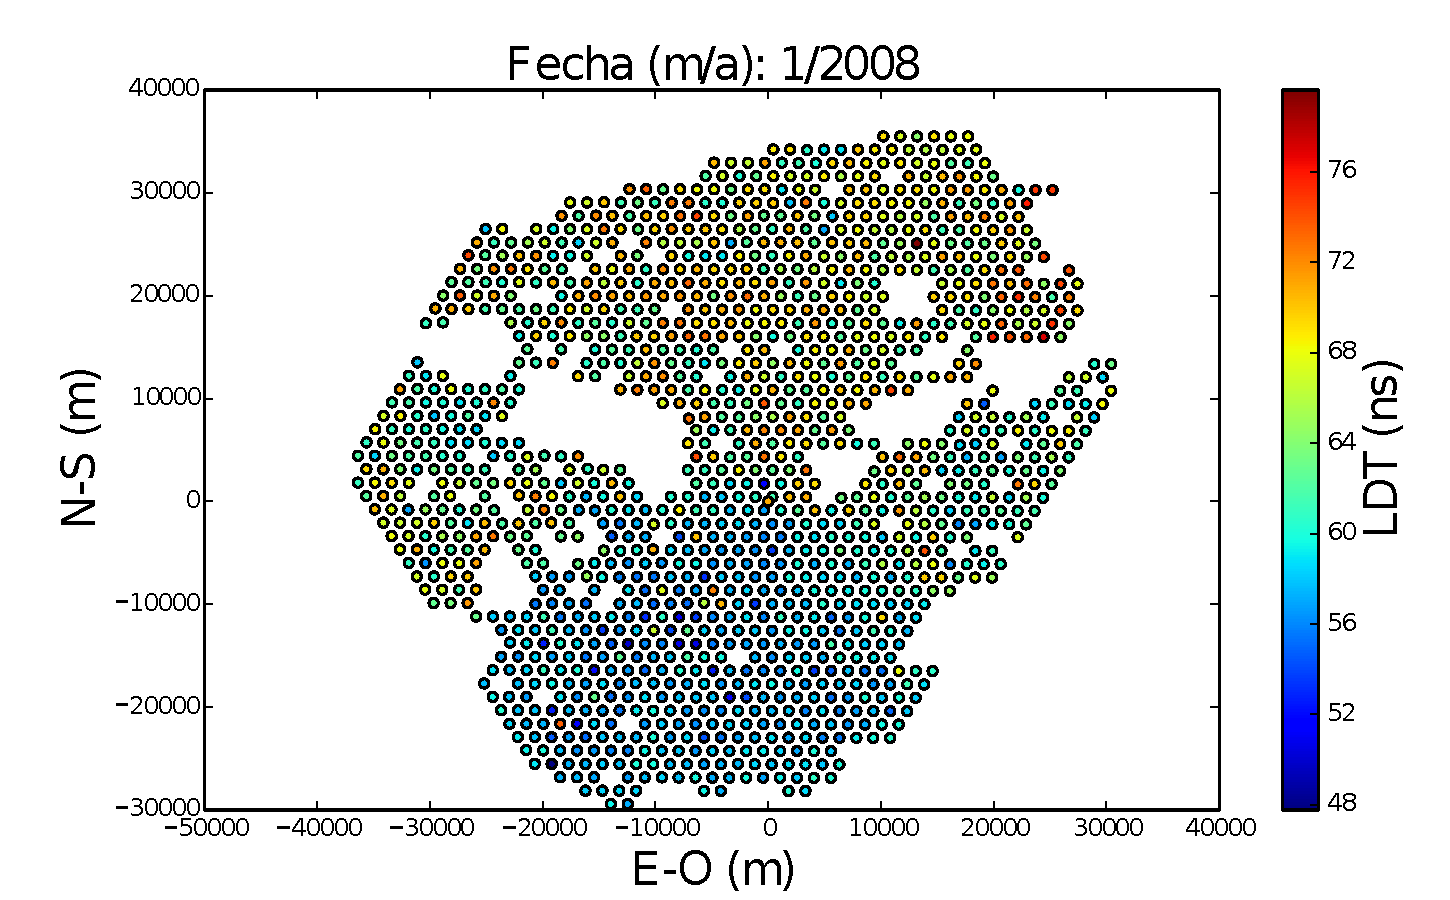
\includegraphics[width=0.67\textwidth]{fig/resultadosAuger/Out_decaytime_main_2008_01} 
			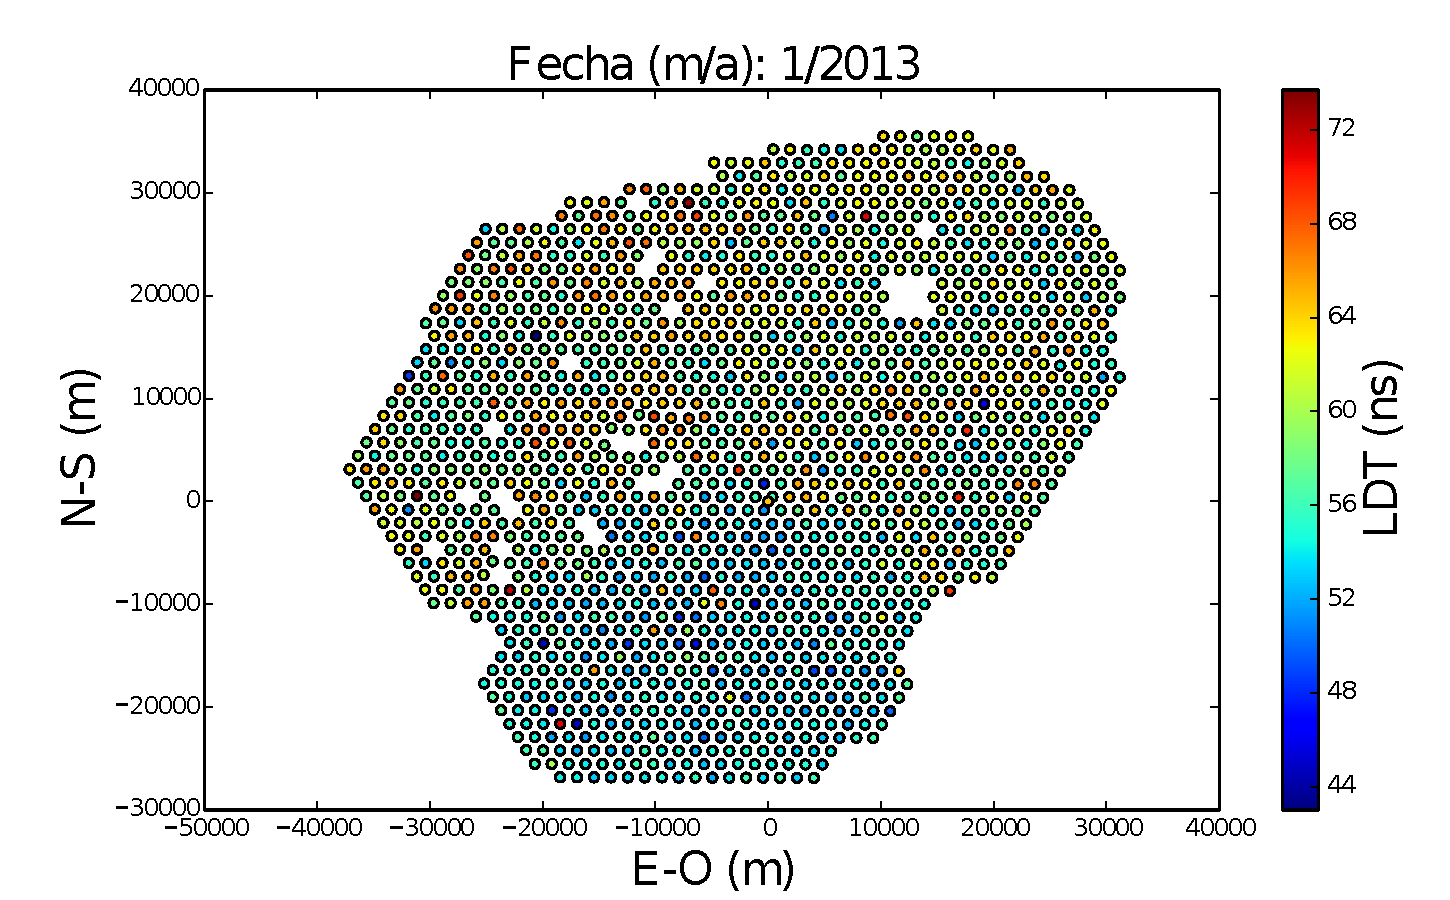
\includegraphics[width=0.67\textwidth]{fig/resultadosAuger/Out_decaytime_main_2013_01}
			\caption{LDT promedio de cada estación para tres estados del detector. La derivación de estos gráficos se explica en el texto.}
			\label{fig:ldtArray}
		\end{center}
	\end{figure}
	%
	Cada una de las estaciones que se grafica participó en el mes de al menos un evento clasificado como T3.
	Para obtener el valor del LDT de cada una se utilizó lo que se denomina el \emph{shape histogram}, que se registra para gada estación que participa de un evento T3.
	Este histograma es el promedio de todas las señales aleatoreas cercanas a \cant{1}{VEM} registradas durante algunos minutos previos a cada evento, es decir, es una suerte de señal elemental promedio.
	Sobre la misma se ajustó un decaimiento exponencial sobre los cuatro bines posteriores al de máxima intensidad (un rango temporal de \cant{100}{ns}) y obtuvo una estimación del LDT.
	Si alguna estación aparece en más de un evento T3 durante el mes, simplemente se promedia los LDT de cada aparición.
	
	Puede observarse en la figura \ref{fig:ldtArray} es que el LDT parece tomar valores similares en las regiones del detector que fueron puestas en operación en momentos cercanos.
	La parte sur del detector, primera en ser desplegada, muestra un color en promedio diferente que la parte norte, instalada algunos años despues.
	También puede notarse que el valor de LDT mínimo del detector (fácilmente apreciable en la escala de color de los gráficos), decreció de manera apreciable con los años, de \cant{\sim54}{ns} en 2005 hasta \cant{\sim44}{ns} en 2003.
	
	Para obtener el efecto de la evolución del LDT en el cálculo de exposure, el único camino posible es resimular la señal que generan las lluvias en las estaciones y un nuevo cálculo de eficiencias.
	Dado que esto es muy costoso computacionalmente, fue necesario elegir un número manejable de detectores representativos.
	Entonces el camino elegido fue despreciar las fluctuaciones locales entre estaciones y simplemente simular algunos \emph{detectores promedio}, que posean un LDT constante que represente el estado del detector durante algún período de tiempo y al mismo tiempo teniendo cuidado de no sobreestimar la exposición.
	
	Para elegir qué detectores promedio simular, se observó la evolución del LDT promedio sobre todo el SD, lo que se muestra en el panel superior de la figura \ref{fig:timeEvolution} junto con su desviación estandar.
	%
	\begin{figure}[h!]
		\begin{center}
			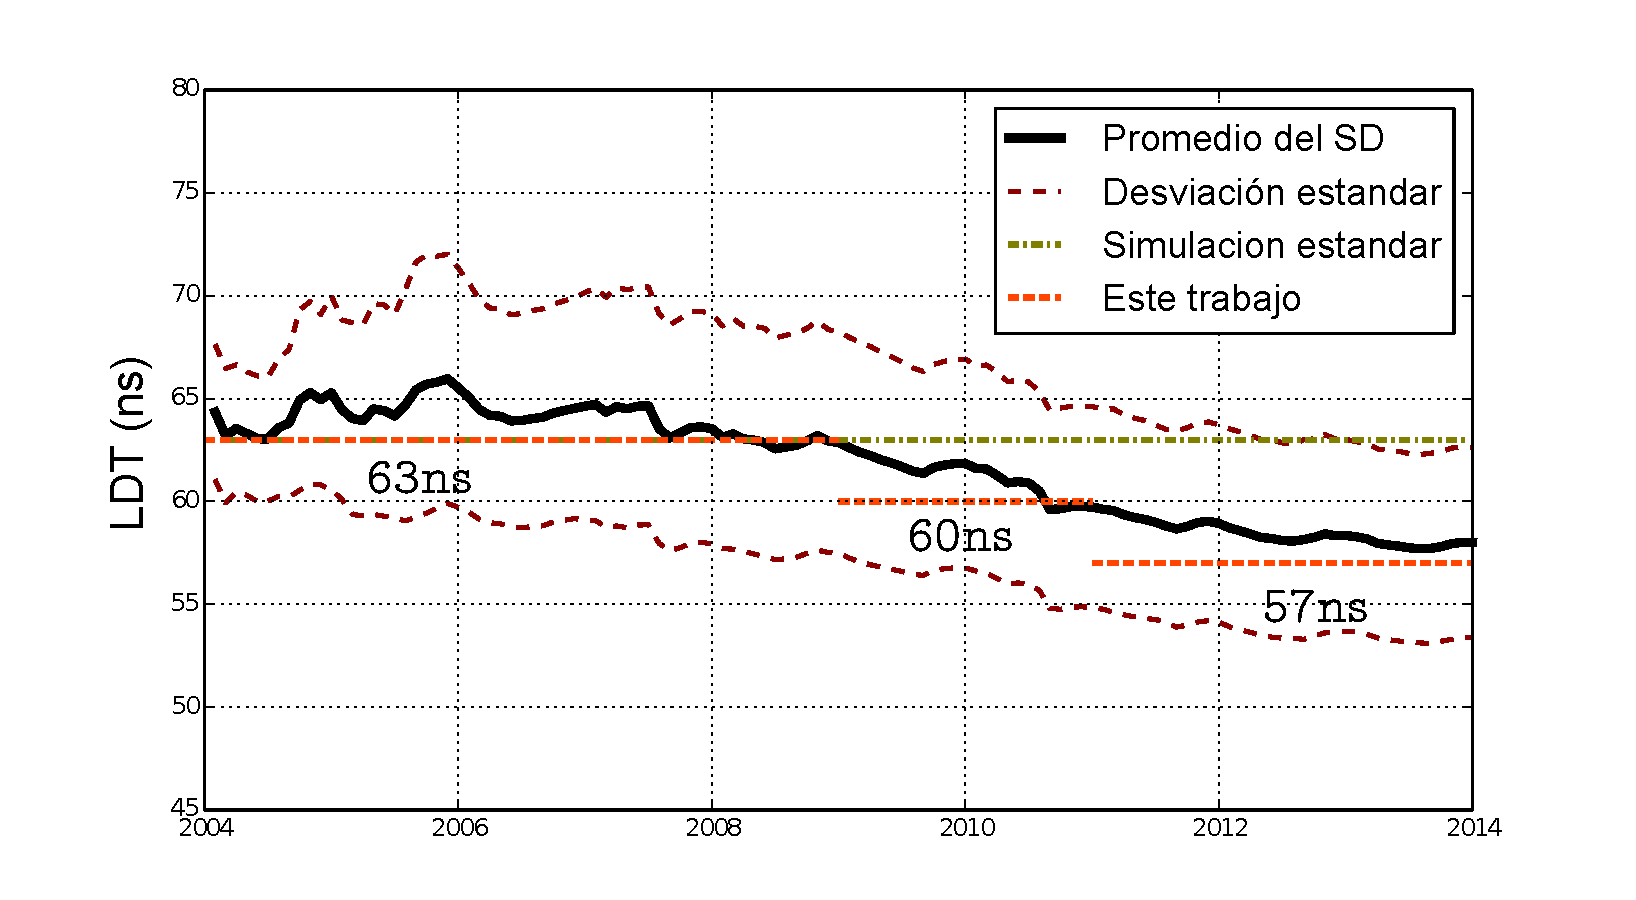
\includegraphics[width=\textwidth]{fig/resultadosAuger/timeEvolution}
			\\ \vspace{0mm}
			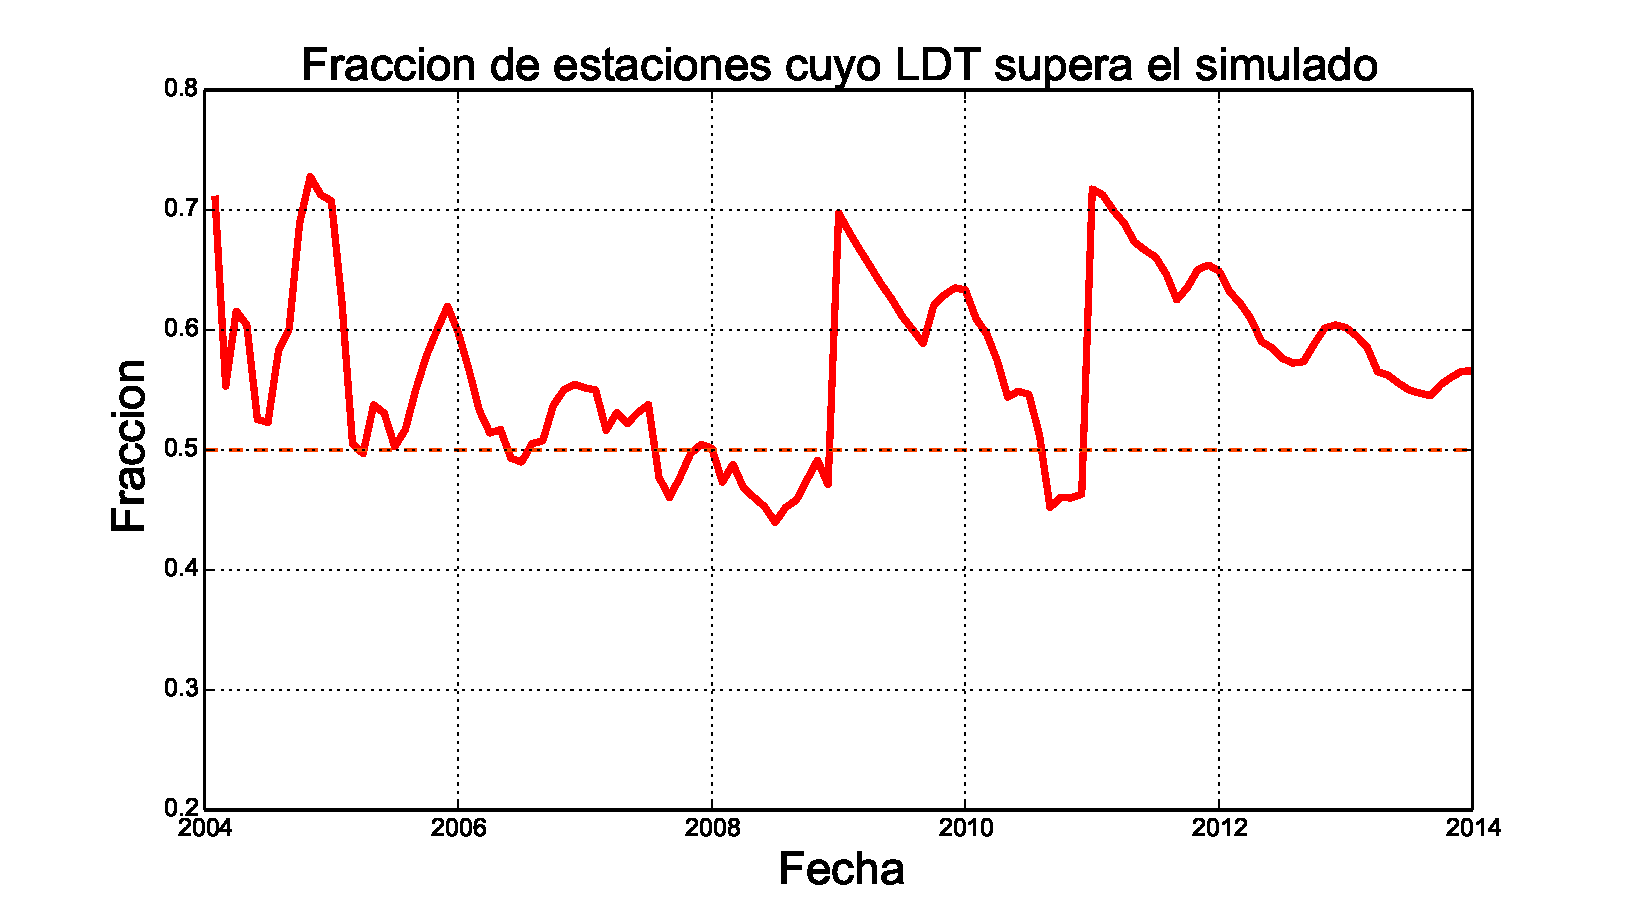
\includegraphics[width=\textwidth]{fig/resultadosAuger/fractionEvolution}
			\caption{Arriba: Evolución del LDT del detector como función del tiempo. La línea negra gruesa marca el promedio del LDT sobre todo el SD y las líneas rojas punteadas su desviación estandar.
			Se señalan además el valor estandar utilizado por \Offline{} y los valores elegidos para representar el detector en los diferentes períodos de tiempo.
			Abajo: Fracción de las estaciones por encima del LDT elegido para simular. La mayor parte del tiempo más del 50$\%$ del detector se encuentra por encima del valor simulado.}
			\label{fig:timeEvolution}
		\end{center}
	\end{figure}
	%
	Se observa en línea negra gruesa que el valor promedio del LDT tiende a decrecer con el tiempo.
	Para contemplar este descenso se eligieron tres valores por debajo del mismo que se utilizó como referencia para simular las eficiencias.
	Los valores elegidos fueron \cant{63}{ns} entre 2004 y 2009, \cant{60}{ns} entre 2010 y 2011 y \cant{57}{ns} desde 2012 en adelante, como se señala en línea punteada en el panel superior de la figura \ref{fig:timeEvolution}.
	Se consideró que estos tres períodos son un buen balance en el compromiso entre representar de manera fiel el detector y no exceder la capacidad de cómputo a la que se tenia acceso.
	Como se observa en el panel inferior de la figura \ref{fig:timeEvolution} la fracción de estaciones por encima del valor elegido supera el 50$\%$ la mayor parte del tiempo.
	
	Una vez definidos los valores de LDT que se quieren representar, fue necesario determinar qué conjunto de valores de tyRef y wAbs utilizar para obtener el LDT deseado.
	Los valores estandar utilizados en \Offline{} son \cant{{\rm wAbs}=100}{m} y tyRef=0.96, con los que se obtiene un valor de \cant{{\rm LDT}=63}{ns}, como se señala en el panel superior de la figura \ref{fig:timeEvolution}.
	Para definir el resto de los valores, se utilizó el mapa LDT(tyRef,wAbs) que se muestra en la figura \ref{fig:timedecay_vs_reflect_absorp}, cedido por Mariangela Settimo~\footnote{ Laboratoire de Physique Nucléaire et de Hautes Energies (LPNHE), Universités Paris 6 et Paris 7, CNRS-IN2P3, Paris, France}.
	%
	\begin{figure}[h!]
		\begin{center}
			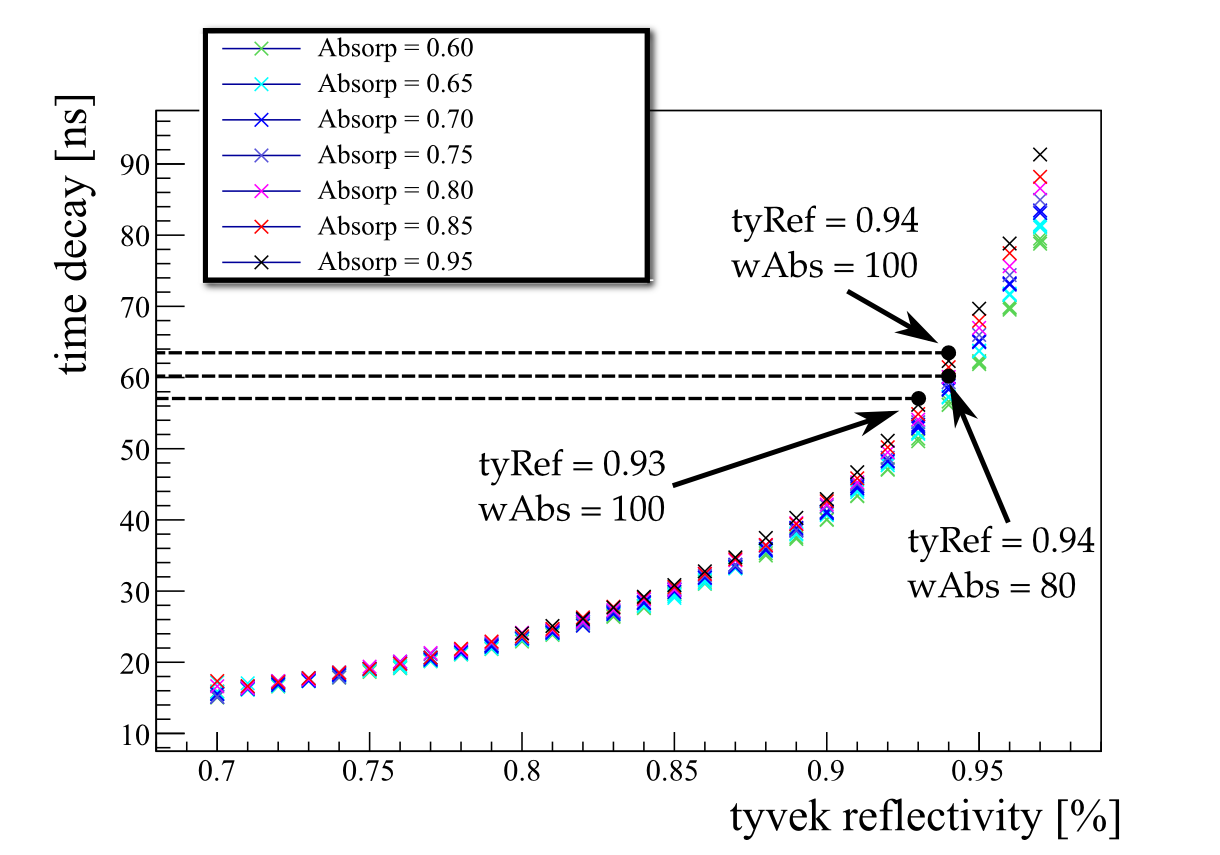
\includegraphics[width=0.9\textwidth]{fig/resultadosAuger/timedecay_vs_reflect_absorp_2}
			\caption{Valor de LDT obtenido con \Offline{} utilizando (tyRef,wAbs) como parámetros de entrada.}
			\label{fig:timedecay_vs_reflect_absorp}
		\end{center}
	\end{figure}
	%
	Para obtenerlo, para cada juego de (tyRef,wAbs) se inyecto en una estación del detector un muón vertical y luego de simular su señal en los PMTs se ajustó sobre la misma un decaimiento exponencial. Luego de realizar el procedimiento del orden de cien veces se obtuvieron los valores promedio que se muestran en la figura.
	Tal como puede observarse, la mayor parte del cambio en el LDT parece deberse a un cambio en la reflectividad del Tyvec, mientras que la absorción del agua implica un cambio de un orden menor\footnote{Se necesita un cambio de un $30\%$ en la absorción del agua para obtener el cambio que sucede al variar 1$\%$ la reflectividad del Tyvec.}.
	Pero por otro lado, existe una degeneración en LDT(tyRef,wAbs), es decir, más de un conjunto (tyRef,wAbs) genera el mismo LDT.
	Debido a la falta de información sobre cuál es la verdadera causa del decenso del LDT en el detector, se decidió variar indistintamente tyRef y wAbs para obtener los LDT que se decidieron simular.
	Estos valores se señalan con línea punteada en la figura \ref{fig:timedecay_vs_reflect_absorp} y se detallan en la tabla \ref{tab:ageingEffect}.
	%
	\begin{table}[h!]
	\centering
	\renewcommand{\arraystretch}{1.4}
	 \begin{tabular}{|l|ccc|c|}
				\hline
				Período       & tyRef & wAbs & LDT        &    Pérdida de exposición \\
				\hline
				$2004 - 2008$ & 0.94  & 100  & $\sim63$ns &    $--$ \\
				$2009 - 2010$ & 0.94  & 80   & $\sim60$ns &    $-15.2\%$\\
				$2011 - 2013$ & 0.93  & 100  & $\sim57$ns &    $-17.5\%$\\
				\hline
	 \end{tabular}
	 \caption{Valores de los parámetros tyRef y wAbs elegidos para representar el estado del detector en los períodos que se detallan en la primer columna. La cuarta columna muestra el valor de LDT que se busca simular mientras que la última muestra la pérdida de exposición que el cambio implica.}
	 \label{tab:ageingEffect}
	\end{table}
	%
	Finalmente, con estos valores se obtuvieron tres juegos de eficiencias que se utilizaron para calcular la exposición en los tres períodos de tiempo correspondientes.
	La última columna de la tabla \ref{tab:ageingEffect} muestra la pérdida de exposición por unidad de tiempo obtenida en el cálculo.
	
	\subsection{Resultado final}
	
	Con todo lo expuesto hasta el momento es posible realizar la integración completa de las ecuaciones \ref{eq:exp4DG} y \ref{eq:exp4ES}, y obtener así las exposiciónes a los distintos canales de detección de neutrinos en Auger, ES, DGH y DGL.
	Sin embargo, dado que hasta la fecha ningún experimento ha detectado neutrinos de energías cercanas al EeV~\footnote{Los neutrinos detectados por IceCube tienen una energía reconstruida 100 veces menor.}, es también interesante calcular la exposición total a neutrinos, es decir, sin importar su dirección de arrivo.
	
	\subsubsection{Exposición total a neutrinos - Combinaci\'on de los análisis}
	
	Antes de obtener la exposición total a neutrinos en Auger, es necesario combinar los análisis, teniendo en cuenta que cada uno puede mejorar la exposición de los demás.
	Si bien cada análisis fue optimizado para identificar neutrinos en cierto rango de ángulo cenital, en principio su sensibilidad puede extenderse más allá del mismo.
	Por ejemplo, un neutrino ES que haya sido rechazado por el criterio de identificación ES por una fluctuación, puede todavia ser aceptado por el criterio de identificación DGH, dado que sus cortes en velocidad son algo más laxos.
	Por otro lado, el criterio de DGH no acepta eventos de 3 estaciones pero pueden ser seleccionados por el criterio ES.
	
	Logicamente, si lo que interesa medir es el flujo de neutrinos sin importar la dirección de la que proviene (flujo difuso), basta con que un evento satisfaga al menos uno de los tres criterios de selección para que sea identificado como neutrino.
	Con esto en mente, en la figura \ref{fig:sketch_combined} se esquematiza la manera correcta de calcular la exposición.
	%
	\begin{figure}[h!]
		\begin{center}
			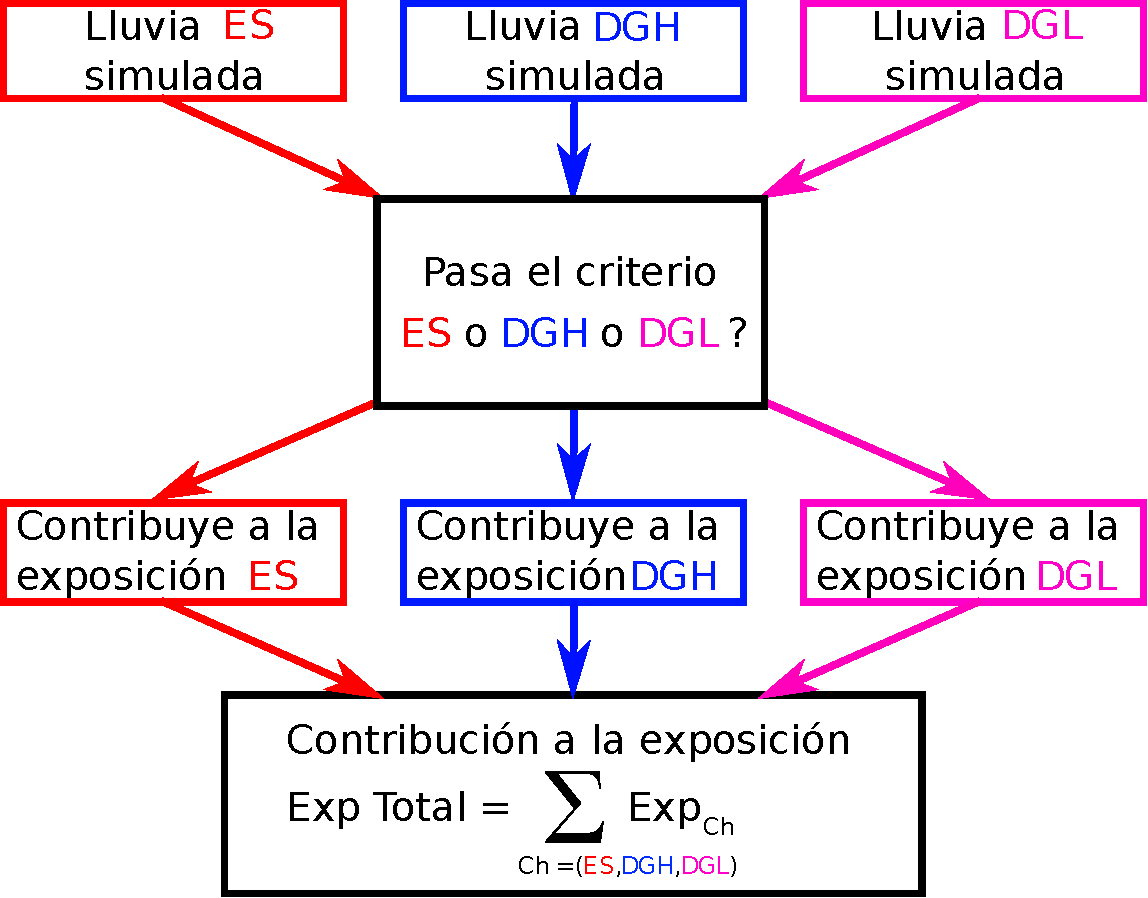
\includegraphics[width=0.65\textwidth]{fig/resultadosAuger/sketch_combined_5}
			\caption{Para calcular la exposición a cada canal es necesario aplicar los tres criterios de selección a todas las lluvias simuladas. En case de ser seleccionada por al menos uno de los tres criterios, dicha lluvia contribuye a la exposición de su canal. Luego La exposición total es la suma de las individuales, como se muestra en la ecuación \ref{eq:expTot}.}
			\label{fig:sketch_combined}
		\end{center}
	\end{figure}
	%
	Al igual que con los datos, cada lluvia simulada, sea ES, DGH o DGL, debe ser evaluada por los tres análisis (criterios de ES, DGH y DGL) y en caso de ser seleccionada por cualquiera de los tres criterios debe constribuir a su correspondiente exposición.
	Luego, una vez obtenidas correctamente las exposiciónes a cada canal, se debe calcular la exposición total a neutrinos con la ecuación \ref{eq:expTot}.
	%
	\begin{equation}\renewcommand{\arraystretch}{2}
	\begin{array}{rcl}
	 N_{esp}& =& N_{esp}^{DGL}+N_{esp}^{DGH}+N_{esp}^{ES} \\
	 & = & \int\limits_{E_\nu}\Phi(E_\nu)~({\cal E}^{DGL}+{\cal E}^{DGH}+{\cal E}^{ES})(E_\nu)~dE_\nu\\
	 & \equiv & \int\limits_{E_\nu}\Phi(E_\nu)~{\cal E}(E_\nu)~dE_\nu
	\end{array}
	\label{eq:expTot}
	\end{equation}
	%
	
	En la figura \ref{fig:expTot} se muestra la exposición del Observatorio para el período completo de medición (1 Enero 2004 - 20 Junio 2013), junto con las exposiciones correspondientes a cada canal. 
	%
	\begin{figure}[h!]
		\begin{center}
			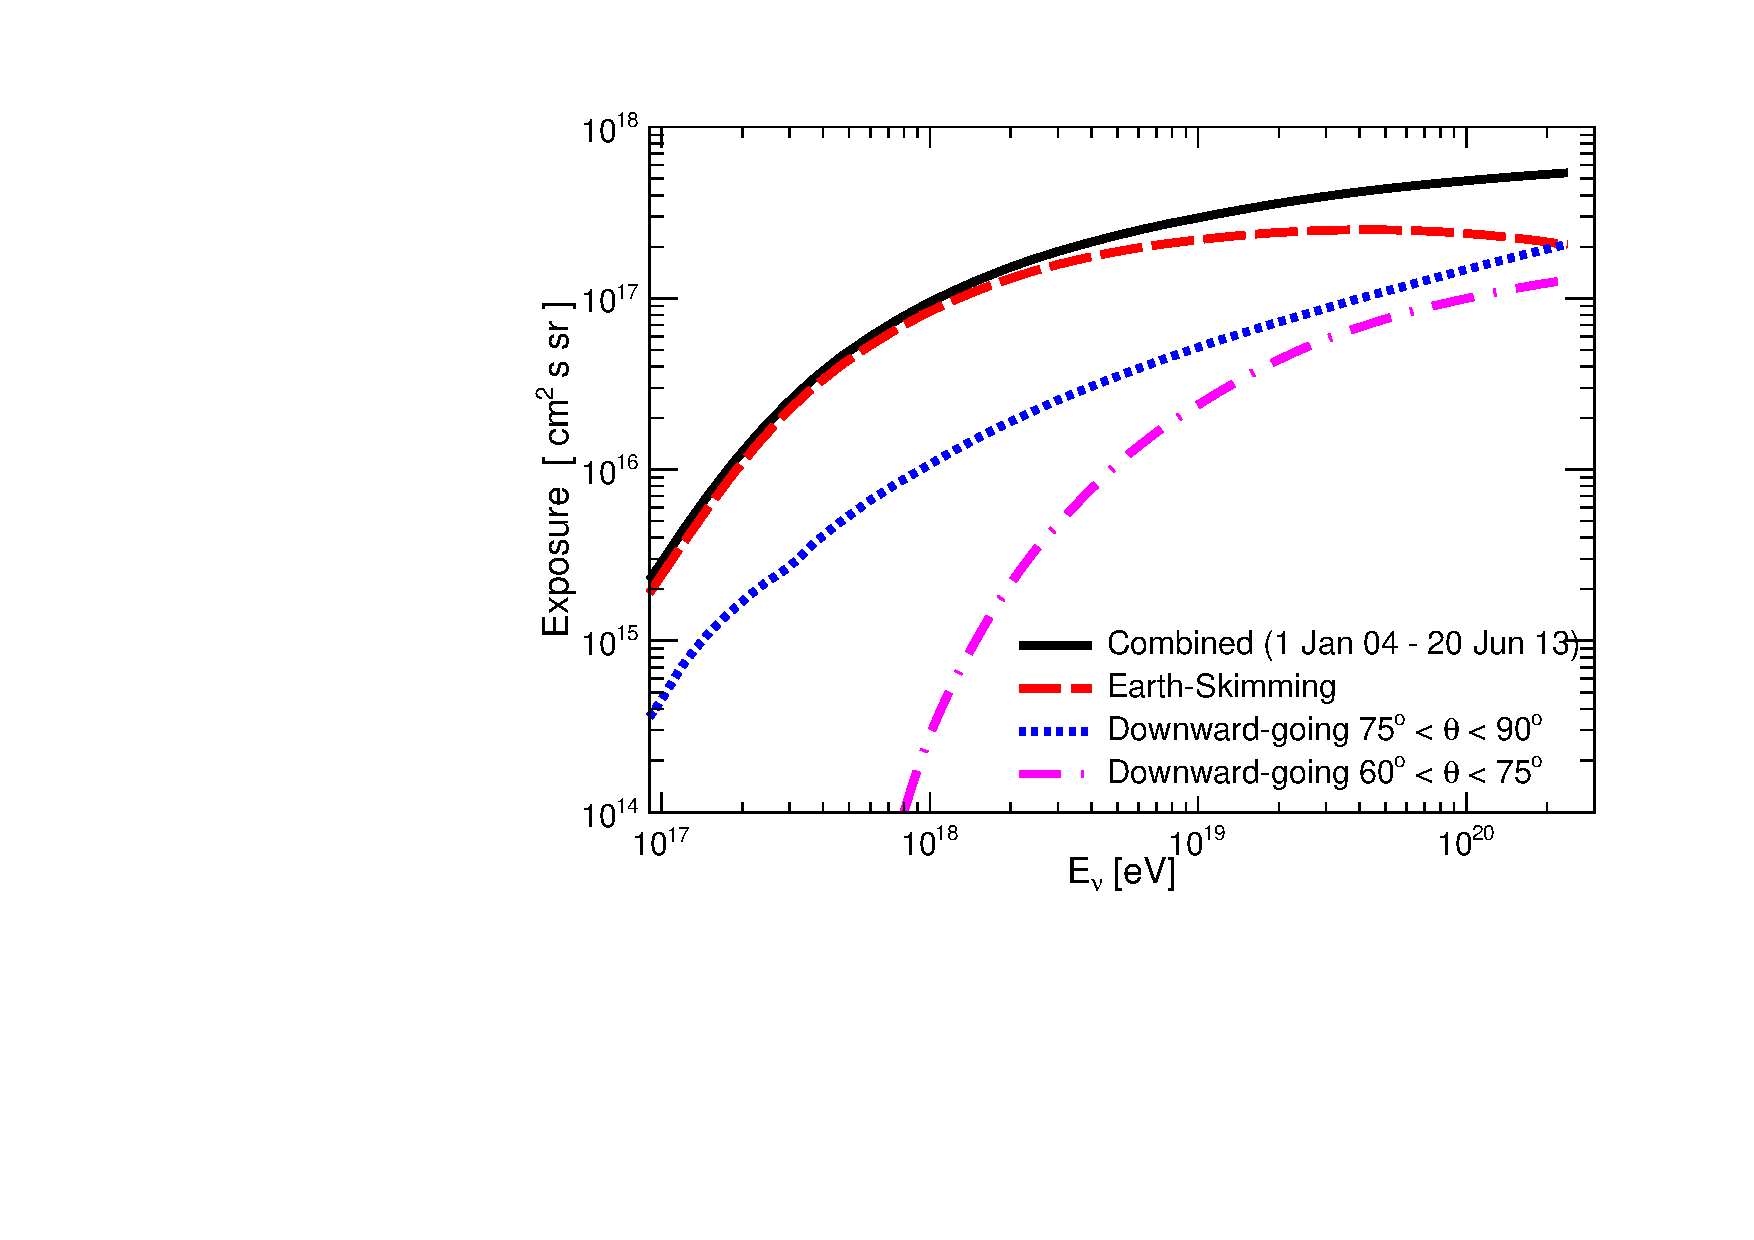
\includegraphics[width=0.9\textwidth]{fig/resultadosAuger/exposure_combined_ageing}
			\caption{Exposición combinada del Observatorio Pierre Auger para el período de medición (1 Enero 2004 - 20 Junio 2013), como función de la energía del neutrino. También se detallan las exposiciones obtenidas para cada canal.}
			\label{fig:expTot}
		\end{center}
	\end{figure}
	%
	A baja energía la exposición es básicamente la del canal ES y los canales DG toman importancia por encima de \cant{E_\nu=10^{18.5}}{eV}.
	
	Es interesante entonces estudiar cuál es la ganancia de aplicar los tres criterios de selección a cada canal de detección.
	En la tabla \ref{tab:expDist} se muestra la distribución de eventos esperados según canal y criterio de selección, en un escenario de $\Phi(E_\nu)\propto E_\nu^{-2}$.
	La última columna de esta tabla muestra la suma de cada fila, es decir, qué cantidad de eventos de cada canal se espera haber detectado.
	%
	\begin{table}[h!]
		\begin{center}\renewcommand{\arraystretch}{1.4}
			\begin{tabular}{|c|c|c|c|c|}
			\hline
			\diagbox{Lluvia}{Criterio} & ES & DGH & DGL  & Total\\ \hline
			ES     &    0.80       &    0.04       &     $<0.001$ & 0.84 \\ \hline
			DGH    &    0.03       &    0.11       &     $<0.001$ & 0.14 \\ \hline
			DGL    &    $<0.001$   &    $<0.001$   &     0.02     & 0.02 \\
			\hline
			\end{tabular}
		\end{center}
		\label{tab:expDist}
		\caption{Distribución de eventos según tipo de lluvia y criterio de selección en un escenario de $\Phi(E_\nu)\propto E_\nu^{-2}$. Los elementos diagonales muestran el efecto de aplicar sólo los criterios de selección optimizados para cada canal. El 93$\%$ de los eventos esperados proviene de los criterios optimizados (suma de la diagonal), mientras que el 7$\%$ restante se gana con la combinación de los análisis. En este escenario, se espera que el 84$\%$ de los eventos detectados correspondan a lluvias ES, el 14$\%$ a eventos DGH y sólo el 2$\%$ a eventos DGL.}
	\end{table}
	%
	Los elementos diagonales de esta matriz representan la fracción de los eventos que se obtiene de aplicar sólo el criterio de selección optimizado para cada canal, mientras que los no diagonales la ganancia que implican los otros criterios.
	De esta, se desprende que el 93$\%$ de los eventos se detectan por los criterios optimizados específicamente\footnote{La suma de los elementos diagonales es $0.80+0.11+0.02=0.93$.} y que la combinación de los análisis implica una ganancia de 7$\%$~\footnote{La suma de los elementos no diagonales es $0.03+0.04=0.07$.}.
	También se muestra que el criterio de DGL no implica ninguna ganancia apreciable a los canales ES y DGH debido a que, por un lado los neutrinos ES tienen chances casi nulas de ser clasificados como eventos DGL y por otro, si bien algunas lluvias DGH pueden ser clasificadas como DGL debido a fluctuaciones en la resconstrucción angular, el peso estadístico de estos eventos es despreciable.
	Del mismo modo, las probabilidades de que una lluvia DGL sea clasificada como ES son despreciables y si bien algunas de las DGL pueden ser clasificadas como DGH, su peso relativo en la exposición total es bajísimo (ver tabla \ref{tab:expDist}).
	
	
	Con el cálculo de la exposición completo también es posible calcular la matriz de clasificación erronea (\emph{missclassification matrix} en inglés) de esta selección.
	Sus elementos dan cuenta de la probabilidad de que un evento identificado por un dado criterio de selección haya sido en realidad iniciado por un evento correspondiente a un canal dado (ver tabla \ref{tab:missclass}).
	%
	\begin{table}[h!]
		\begin{center}
		\renewcommand{\arraystretch}{1.4}
			\begin{tabular}{|c|c|c|c|c|c|}
			\hline
			\diagbox{Lluvia}{Criterio} & ES $\wedge$ DGH &  ES    &  DGH   &  DGL      \\ \hline
			ES                         & 0.90            &  0.86  &  0.48  &  0.00     \\ \hline
			DGH                        & 0.10            &  0.14  &  0.52  &  0.03     \\ \hline
			DGL                        & 0.00            &  0.00  &  0.00  &  0.97     \\ \hline\hline
			Probabilidad               & 0.69            &  0.20  &  0.09  &  0.02     \\
			\hline
			\end{tabular}
		\end{center}
		\label{tab:missclass}
		\caption{Matriz de clasificación erronea (\emph{missclassification matrix} en inglés). La última fila representa la probabilidad de aparición de cada tipo de clasificación. De los eventos identificados como neutrinos, se espera en el 69$\%$ de los casos una clasificación ES y DGH simultánea, mientras que en el 20$\%$ sólo ES, en el 9$\%$ clasificación DGH y en el 2$\%$ DGL. En caso de que un evento sea ES $\wedge$ DGH se espera que el 90$\%$ realmente sea ES y el 10$\%$ restante DGH. Las clasificaciones ES serán 86$\%$ lluvias ES y el 14$\%$ DGH. Un evento etiquetado como DGH será en el 52$\%$ realmente DGH y el 48$\%$ restante ES. Por último el 97$\%$ de los eventos DGL seran realmente DGL mientras que el 3$\%$ restante serán DGH mal clasificados.}
	\end{table}
	%
	En esta se muestra como se espera que el 69$\%$ de los eventos sean clasificados como eventos ES y DGH simultaneamente, el 20$\%$ ES, el 9$\%$ DGH y el 2$\%$ DGL.
	En caso de clasificación simultánea de los canales ES y DGH, el 90$\%$ de los casos corresponderá a eventos iniciados por neutrinos ES mientras que el 10$\%$ restante a lluvias DGH. 
	Si se tuviera un evento sólo clasificado como ES, el 86$\%$ de los mismos correspondería a lluvias ES y el 14$\%$ restante a lluvias DGH.
	En cambio si se registrara un evento clasificado como DGH, el 52$\%$ de las veces provendrá de una lluvia DGH, mientras que el 48$\%$ restante corresponderá a lluvias ES. 
	Si bien esto podría parecer llamativo, no hay que perder de vista que se esperan sobre el detector al rededor de 8 veces más eventos ES que DGH.
	Por último, el 97$\%$ de los eventos clasificados como DGL habran sido iniciados por lluvias DGL mientras que el 3$\%$ restante serán DGH mal clasificados.
	
	
% 			ES & 0.951 & 0.048 & despreciable \\ \hline
% 			DGH & 0.195 & 0.804 & despreciable \\ \hline
% 			DGL & despreciable & despreciable & 0.999 \\
%	0.84:0.14:0.02
%	
%           &    ES crit    &    DGH crit    &     DGL crit
% ES sh     &    0.789      &    0.042       &     neglect.
% DGH sh    &    0.027      &    0.112       &     neglect.
% DGL sh    &    neglect.   &    neglect.    &     0.020
% 	you are right, these numbers are important. I will work on that after the ICRC. For the moment I can only give you the exposure contribution (gain) in an E^{-2} scenario matrix, and it looks like:
% 
%           &    ES crit    &    DGH crit    &     DGL crit
% ES sh     &    0.695      &    0.035       &     neglect.
% DGH sh    &    0.045      &    0.185       &     neglect.
% DGL sh    &    neglect.   &    neglect.    &     0.04
% 
% please take into account that we have a systematic error of 40%. 
% for instance, from the table you can see that 3.5% of the total limit to an E^-2 flux is due to simulated 
% ES neutrinos selected by the DGH analysis. This gives an idea of the probability of "missclassification", but its no so simple, since the most of the ES simulated neutrinos that passes ES crit, also passes the DGH crit with a high reconstructed angle...
% In any case, if any of the three analysis finds a candidate we will have to scrutinize it with as many eyes 
% as possible and try to (1) make sure it is a neutrino and not a detector fluke, and (2) identify it as ES or 
% Down-Going quasi-horizontal, something that might not be that easy.
	
\section{Errores sistem\'aticos}
\label{sc:systErr}

El cálculo de la exposición descripto el la sección \ref{sc:expoNu} involucra una gran cantidad de factores. 
Algunos de ellos, como la sección eficaz neutrino nucleón, las pérdidas de energía del \tauon{} en la tierra o el modelo hadrónico, no son conocidos con precisión y la comunidad científica convive con una variedad de opciones a las que asigna un similar grado de creencia.
Entonces es importante entonces estimar la incerteza sistemática asociada a la particular selección de ingredientes utilizados y a los programas elegidos para llevar a cabo la simulación.
En este contexto, es útil clasificar las elecciones realizadas en las siguientes categorías:
%
\begin{itemize}
 \item \textbf{Simulaciones de Monte Carlo:} algunos de los pasos de las simulaciones Monte Carlo descriptas en el capítulo \ref{ch:simulacionAuger} se basan en modelos que describen física que no se conoce con detalle.
 \item \textbf{Sección eficaz $\nu$--nucleón y pérdida de enería del \tauon{}:} sus valores no han sido medidas a estas energías y existen extrapolaciones alternativas a las adoptadas en este trabajo.
 \item \textbf{Flujo de $\tau$s desde las montañas:} su incerteza está dominada por la elección del modelo de sección eficaz $\nu$--nucleón y de propagación del $\tau$ en la roca.
\end{itemize}
%
El objetivo de ésta sección es describir la estrategia utilizada para estimar la incerteza asociada a cada una de estos grupos y discutir su propagación al resultado final.

	\subsection{Método de estimación}
	
	Para obtener una estimación del error sistemático inducido por un dado ingrediente, $X$~\footnote{$X$ podría ser por ejemplo la lista productos de la interacción $\nu$--nucleón, que impacta en las eficiencias, o el modelo de pérdida de energía del \tauon{} en la tierra, que cambia el el factor $P(E_\tau|E_\nu,\theta)$ en la ecuación \ref{eq:exp5ES}.}, para los tres análisis se utilizó el mismo procedimiento.
	Se reevaluó la exposición modificando uno o varios de los parámetros que cambian $X$ y se la comparó con la de referencia, obteniendo así una estimación de magnitud porcentual que puede alcanzar un cambio en dicho ingrediente.
	Luego, dado que la evaluación de estos errores se encuentra limitada por el repertorio de modelos o programas que existen en la actualidad, en lugar calcular la desviación estandar respecto de la exposición de referencia para cada fuente de error, se utilizó como estimadores del error sistemático a los valores más optimista y más pesimista de entre todos los calculados para dicha fuente.
	
	Por otra parte, una comparación exhaustiva que incluya la reevaluación de la exposición en todo el espacio de parámetros requeriría generar ${\cal O}(10^7)$ eventos simulados\footnote{Las librerías de eventos generadas para las búsquedas de neutrinos en Auger tienen ${\cal O}(10^6)$ eventos en total.}. 
	Este procedimiento es claramente impracticable y fue necesario buscar una alternativa.
	El camino elegido fue el de restringir la comparación a una pequeña región representativa del espacio de parámetros. 
	La filosofía para determinar dicha región representativa fue la misma en los trés análisis: elegir entre los bines que representen la mayor parte de la sensitividad en la búsqueda, los que más posibilidades tengan de ser afectados por las fuentes de los sistemáticos.
	En particular, para el análisis de DGL se utilizó tres energías (\cant{0.3}{EeV},\cant{1}{EeV},\cant{3}{EeV}), de las que se resimuló los ángulos más cercanos a DGH todo el rango de profundidades \cite{tesisNavarro}.
	Por otro lado, en DGH se consideró suficiente utilizar \cant{E_\nu=1}{EeV} y $\theta=85^\circ$ \cite{tesisJavier}.
	Finalmente en el análisis de ES se resimuló los bines que se detallan en la figura \ref{fig:importantBins_oldWeights}~\cite{tesisYann}.
	%
	\begin{figure}[h!]
		\begin{center}
			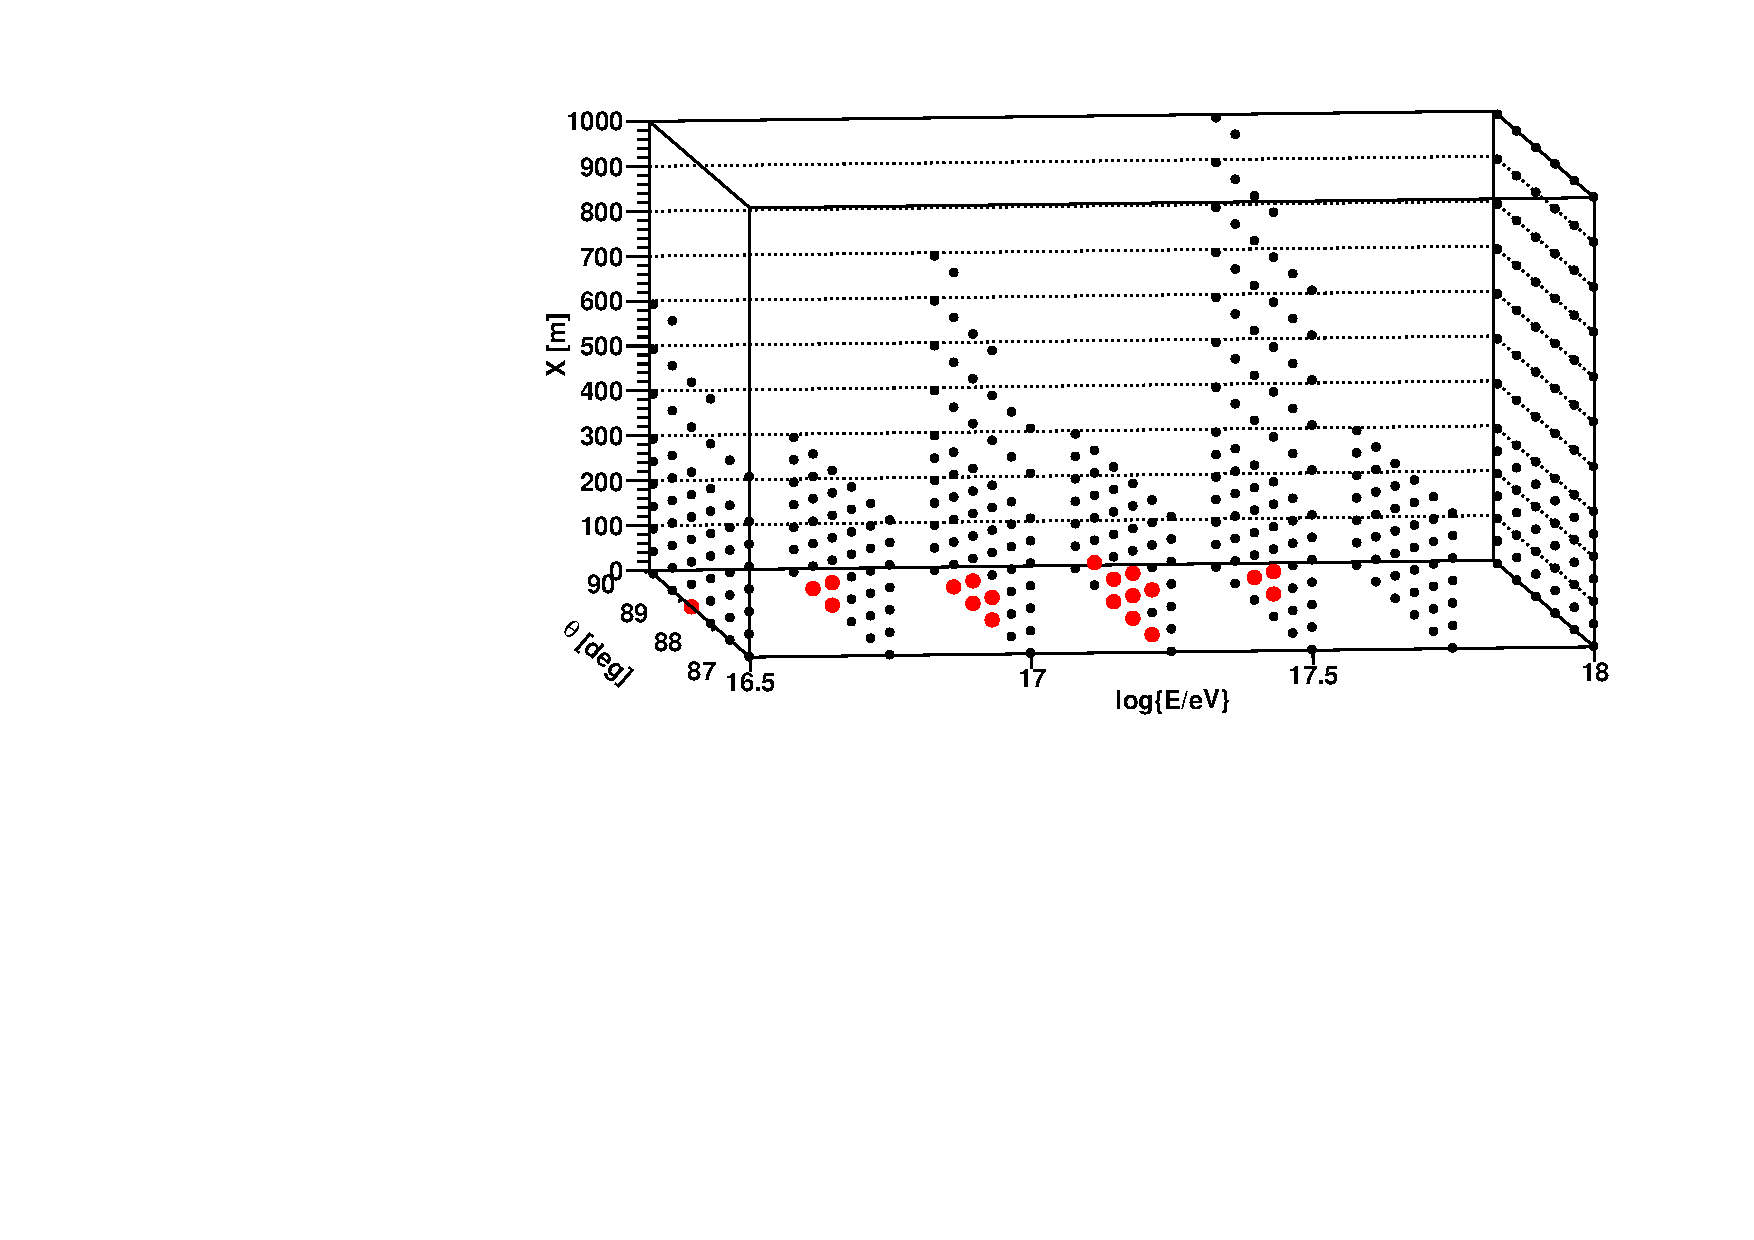
\includegraphics[width=0.75\textwidth]{fig/resultadosAuger/importantBins_oldWeights}
			\caption{Lluvias simuladas para el análisis de ES. En rojo se señalan los bines utilizados para el cálculo de errores sistemáticos.}
			\label{fig:importantBins_oldWeights}
		\end{center}
	\end{figure}
	
	\subsection{Error asociado a las simulaciones de Monte Carlo}
	
	Este grupo incluye el generador de la interacción primaria en los canales DG, la parametrización de las PDFs (parton distribution function) en dicho generador, el simulador de EAS elegido y algunos de sus parámetros como el modelo hadrónico y el nivel de thinning.
	
		\subsubsection{Generador de la interacción primaria}
		
		Este sistemático aplica solo a los canales DG.
		Tanto en DGL como en DGH se utilizó como referencia \herwig{} 6.5.10 \cite{herwigRef} y se comparó con {\sc PYTHIA}\cite{pythia} y {\sc HERWIG++} \cite{herwig++}.
		La incerteza sistemática asociada a esta fuente es de \eband{2.6}{3.7} para DGL y de \eband{0}{7} en DGH.
		
		\subsubsection{Función de distribución de partones}
		
		Tanto \herwig{} como {\sc PYTHIA} ofrecen la posibilidad de elegir entre varias parametrizaciones de las PDFs o incluso utilizar un modelo externo.
		Para evaluar esta fuente de sistemático en DGH se utilizó el modelo CTEQ06m~\cite{CTEQ06m} y en DGL el modelo MRST98~\cite{MRST98}.
		Luego de una comparación exhaustiva contra las posibilidades ofrecidas, la incerteza obtenida para las distribuciones partónicas fue de \eband{2}{7} en DGH y \eband{4}{5} en DGL.
		
		\subsubsection{Simulador de EAS y algoritmo de thinning}
		
		Además de \aires{}, se recalculó el resultado en las lluvias DG utilizando {\sc CORSIKA} \cite{corsika}.
		De esta reevaluación se obtuvo una pérdida de exposición del 17$\%$ para {\sc CORSIKA} respecto de \aires{}.
		Por lo que se cita un error de \eband{0}{17} para DGH y \eband{17}{0} para DGL, en el que la exposición de referencia se calculó utilizando {\sc CORSIKA}.
		
		Respecto de esta fuente, para el análisis de ES no fue posible estimar el sistemático debido a que {\sc CORSIKA} no permite simular eventos ascendentes. 
		%auger.in2p3.fr/DPA/minutes/mal00N/accomparison2.ps
		
		Otro parámetro importante a la hora de simular la evolución de las lluvias atmosféricas es el nivel de thinning, que determina el detalle con el que se simulan las partículas de baja energía.
		Para los tres análisis se utilizó como referencia un factor de $10^{-6}$ y se lo comparó con simulaciones más detalladas, utilizando un factor de $10^{-7}$.
		Los valores obtenidos fueron \eband{0.3}{0} para ES y \eband{7}{0} para DGH y DGL.
		
		\subsubsection{Modelo hadrónico}
		
		Otra fuente de incerteza en el proceso de simulaciónde la lluvia atmosférica reside en la elección del modelo utilizado para calcular las interacciones hadrónicas.
		Estos modelos ajustan sus parámetros para reproducir los datos obtenidos en aceleradores a bajas energías, por lo que la simulacion de lluvias atmosféricas de altas energías requieren su extrapolación.
		Para obtener el error sistemático asociado a esta fuente se utilizó como referencia el modelo QGSJETII \cite{qgsjetii} y se comparó el resultado con QGSJET \cite{qgsjet} y SYBIL \cite{sybil}.
		El resultado obtenido fue \eband{4.7}{1} en ES, \eband{5}{2} en DGH y \eband{0}{6} en DGL.
		
	\subsection{Error asociado a la sección eficaz neutrino nucleón y a las pérdidas de energía del tauón}
	
	Para los canales DG se utilizó la sección eficaz junto con su incerteza asociada calculada por Sarkar en \cite{sarkarNuxSec}.
	Al propagar el cálculo hacia la exposición se obtuvo una \eband{9}{9} en DGH y \eband{7}{7} en DGL.
	Es importante resaltar que este resultado es compatible con nuevas extrapolaciones de las funciones de distribución de partones publicadas recientemente \cite{newPDFs}.
	
	Este procedimiento no pudo llevarse a cabo en el análisis de ES dado que un cambio en la sección eficaz implica la resimulación del término $f(E_\tau|E_\nu,\theta)$ (ver sección \ref{sbsbsc:sim_prop_tierra}).
	
	\begin{figure}[h!]
		\begin{center}
			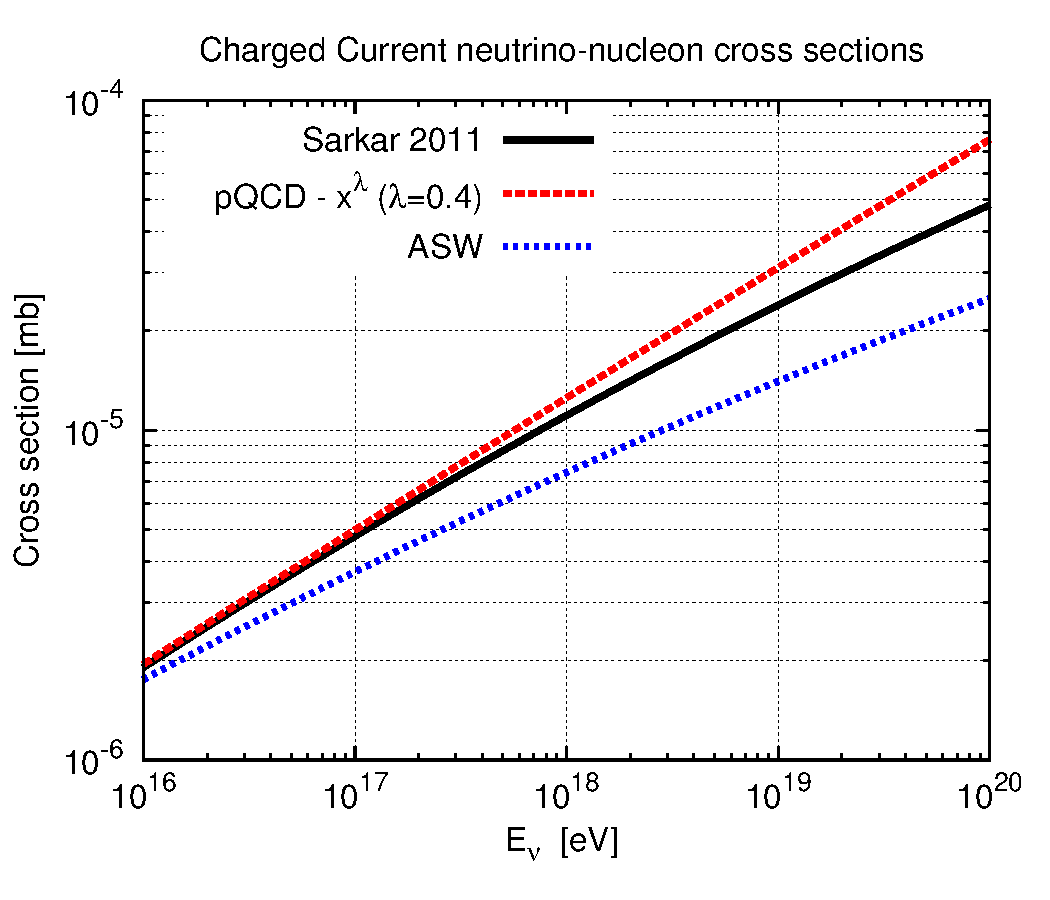
\includegraphics[width=0.65\textwidth]{fig/resultadosAuger/nu_xsection_models}\\
			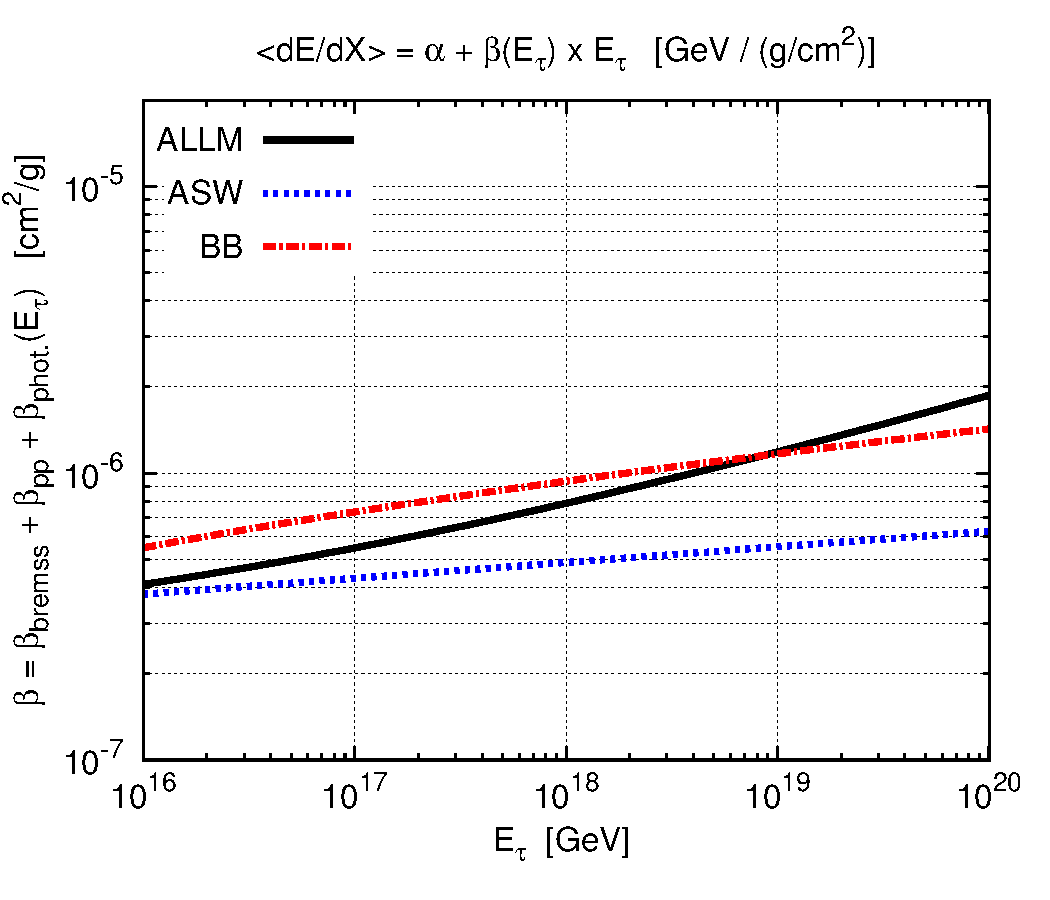
\includegraphics[width=0.65\textwidth]{fig/resultadosAuger/tau_E_loss_models}
			\caption{asd}
			\label{fig:crossSectionSist}
		\end{center}
	\end{figure}
	
	
	\subsection{Error asociado a la topografía }
	
	\subsection{Combinación de las incertezas de cada análisis}
	
	
	
	\begin{table}[h!]
	\centering
	\renewcommand{\arraystretch}{1.4}
	\footnotesize
	\newcolumntype{C}[1]{>{\centering\arraybackslash}p{#1}}
		\begin{tabular}{|C{0.2\textwidth}|c|c|c|c|}
		\hline
		Fuente del  & ES        & DGH       & DGL        & Combined         \\
		sistemático & ($90^\circ,95^\circ$) & ($75^\circ,90^\circ$) & ($65^\circ,75^\circ$) & ES / DGH / DGL   \\
% 		\hline
% 		& {\tiny \bf GAP 2013-100}     & \multirow{2}{*}{\tiny \bf PRD 84, 2011}    &   \multirow{2}{*}{\tiny \bf GAP2013-013} & \multirow{2}{*}{\tiny \bf 83.9\% / 13.7\% / 2.4\% }\\
% 		& {\tiny \bf PRD 79, 2009}     &     &  &  \\
		\hline
		
		Gen. de interacción primaria    &  no apl. &   0\%, -7\%     &   +3\%, -4\%  & +0.07\%, -1.0\% \\
		
		\hline
		
		PDF en el generador             &  no apl. &   0\%, -7\%     &   +4\%, -5\%  & +0.1\%, -1.0\% \\
		
		\hline
		
		Simulador de EAS                &  no eval. &   0\%, -17\%    &   +17\%, 0\%  & +0.4\%, -2.3\% \\
		
		\hline
		
		Modelo hadrónico                & +4.7\%, -1\%      &  +5\%, -2\%     &   +0\%, -6\%  & +4.6\%, -1.3\% \\
		
		\hline
		Algoritmo de thinning           & +0.3\%, 0\%   &  +7\%,  0\%     &   +7\%,  0\%  & +1.1\%, -0.0\% \\
		\hline
		\hline
		{\bf $\bm{ \sigma_{\nu_\tau}\ \otimes\ \tau}$ E-loss}    & \multirow{2}{*}{\textcolor{Red}{+40\%, -33\%}}  & \multirow{2}{*}{+9\%, -9\%}  & \multirow{2}{*}{+7\%, -7\%} & \multirow{2}{*}{\bf +33.6\%, -27.7} \\
		$\sqrt{H^2+I^2}$                                     &                 &                 &             & \\
		\hline
		\hline
% 				%%%%%%%%%%%%%%%%%%%%%%%%%%%%%%%%%%%%%%%%%%%%%%%%%%%%%%%%%%%%%%%%%%%%%%%%%%%%%%%%%%%%%%%%%%%%%%%%%%
		{\bf Topography} 	                            &  +18\%, 0\%    & +20\%, 0\% & not apl.   & +18.9\%, 0\%  \\

		\hline
		\hline
		{\bf Total}                     &  \multicolumn{3}{c|} {}  & {\bf +38.8\%, -27.9\%}         \\
		\hline
		%%%%%%%%%%%%%%%%%%%%%%%%%%%%%%%%%%%%%%%%%%%%%%%%%%%%%%%%%%%%%%%%%%%%%%%%%%%%%%%%%%%%%%%%%%%%%%%%%%
		\end{tabular}
		\caption{}
		\label{tab:sist}
	\end{table}

\section{Analisis ciego}

	\subsection{Abriendo la caja}
	
	\subsection{L\'imite al flujo difuso y diferencial}
	\begin{figure}[h!]
		\begin{center}
			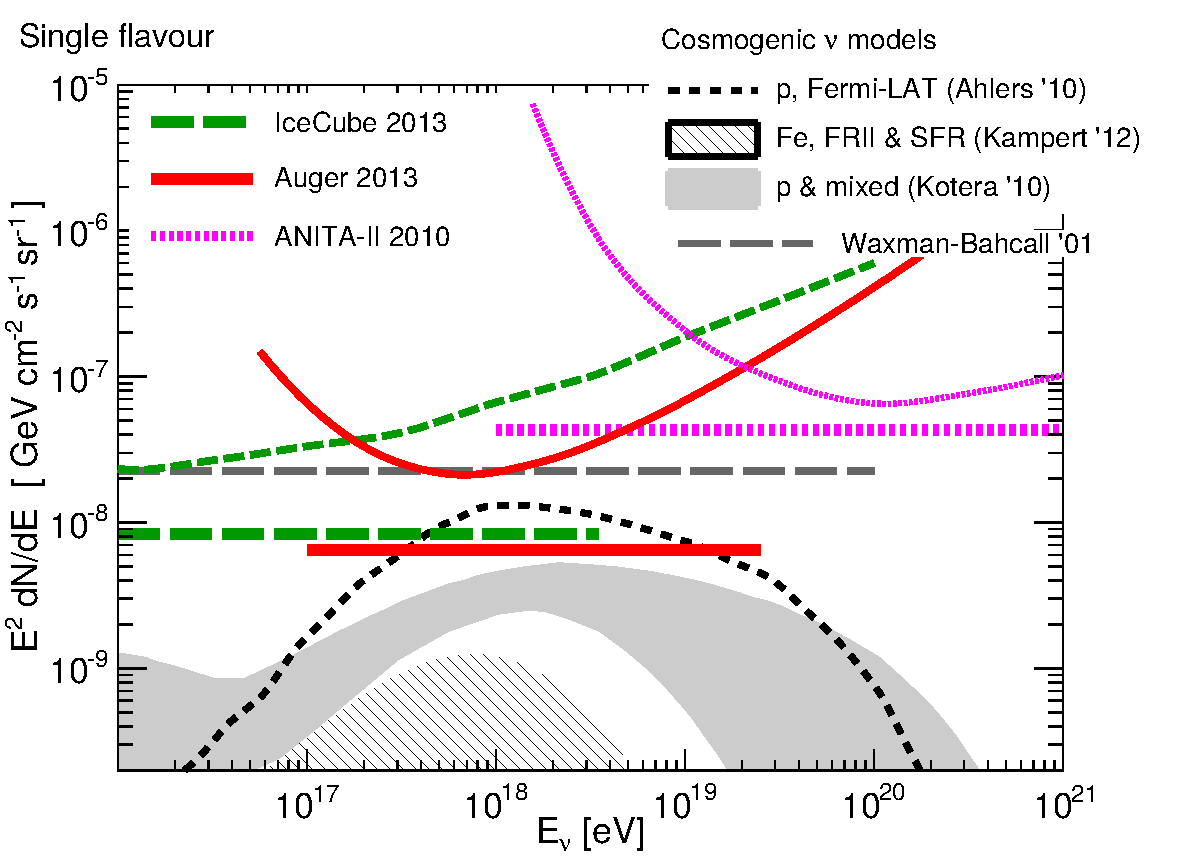
\includegraphics[width=0.9\textwidth]{fig/resultadosAuger/limits_combined_ageing}
			\caption{asd}
			\label{fig:}
		\end{center}
	\end{figure}
	
	\begin{table}[h!]
		\begin{center}
		\renewcommand{\arraystretch}{2.0}
			\begin{tabular}{|c|c|} 
			\hline
			Diffuse flux       &  Expected number of events   \\
			Neutrino Model     &  (1 Jan 04 - 20 Jun 13)   \\
			\hline
			\hline
			Cosmogenic (Kampert {\it et al.}) - proton, FRII      &  \textcolor{Red}{$\sim$ 4.0}  \\
			\hline
			Cosmogenic (Ahlers {\it et al.}) - proton, Fermi-LAT  &  \textcolor{Red}{$\sim$ 3.2}  \\
			\hline
			Cosmogenic (Kampert {\it et al.}) - proton, SFR       &  \textcolor{Blue}{$\sim$ 0.9}  \\
			\hline
			Cosmogenic (Kotera {\it et al.}) - band               &  \textcolor{Blue}{$\sim$ 0.5 $-$ 1.4}  \\
			\hline
			Cosmogenic (Kampert {\it et al.}) - iron, FRII        &  $\sim$ 0.3  \\
			\hline
			\end{tabular}
		\end{center}
	\end{table}
	

	
	\begin{figure}[h!]
		\begin{center}
			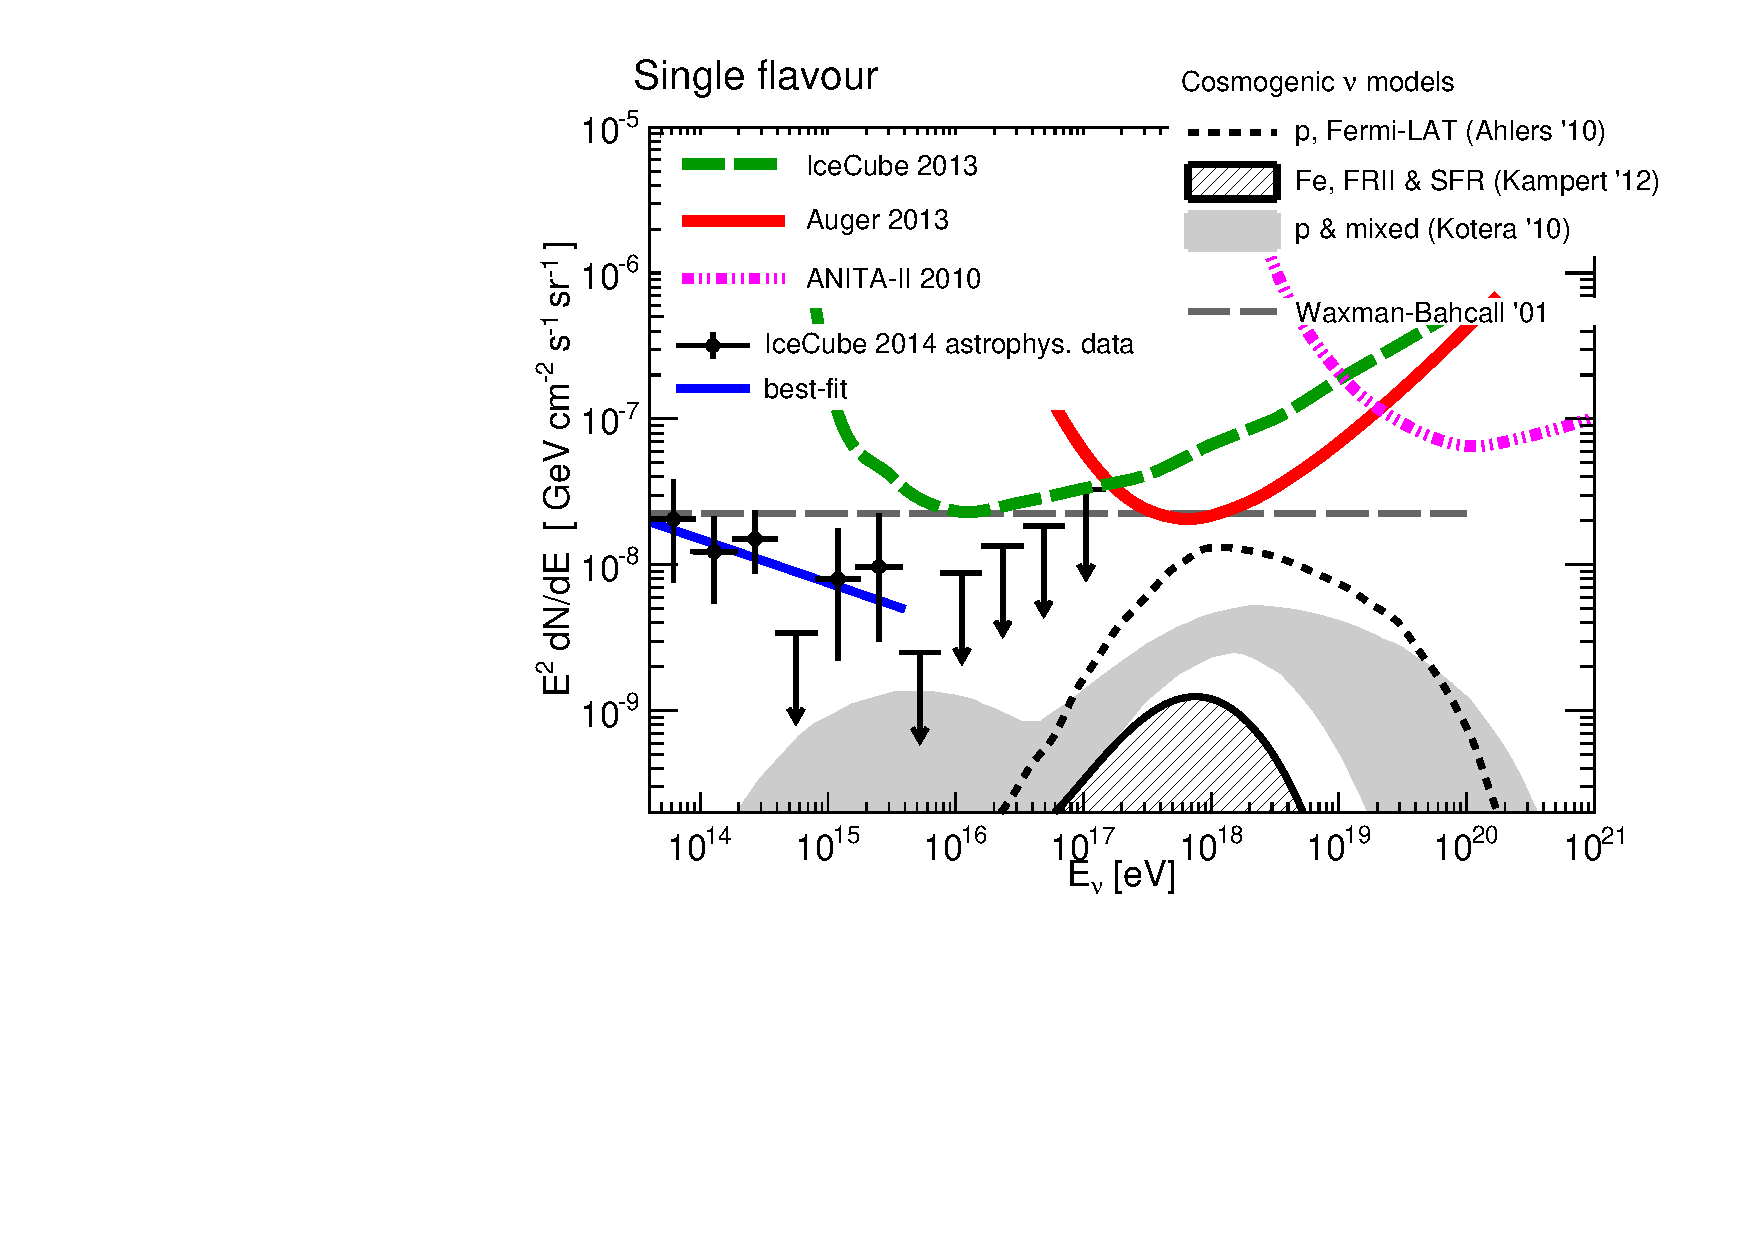
\includegraphics[width=0.9\textwidth]{fig/resultadosAuger/diff_limits_and_many_models_IceCube_data_noextrap}
			\caption{asd}
			\label{fig:}
		\end{center}
	\end{figure}

	
	